\documentclass[a4paper,11pt]{report}
\usepackage[utf8]{inputenc}
\usepackage[english]{babel}
\usepackage{amsmath,amssymb,graphicx,setspace,hyperref}
\usepackage[T1]{fontenc}
\usepackage{cite}
\usepackage{booktabs}
\graphicspath{{figures/}{../THGNN/data/plots/}{../comparison_results/}{../stock_analysis_results/}}
\setcounter{tocdepth}{3}
\setcounter{secnumdepth}{3}

% \usepackage{charter} 
 \renewcommand{\rmdefault}{bch} 
 
%hyperlinking references and table contents
\hypersetup{
colorlinks=true,
linkcolor = black,
filecolor = black,
urlcolor = black, 
citecolor = blue}
 
\onehalfspacing
\widowpenalty=10000
\clubpenalty=10000


\addtolength{\voffset}{-0.6cm}
\addtolength{\textheight}{0.8cm}
\addtolength{\hoffset}{-0.7cm}
\addtolength{\textwidth}{1.4cm} 
\addtolength{\marginparwidth}{1.2cm}




\begin{document}

\fontsize{11}{15}\selectfont
% \fontsize{x}{y}
% x: font size
% y: baseline (font size + space between lines)

\pagestyle{empty}

\thispagestyle{empty}
\begin{center}
\textbf{\Large Graph-Structured Deep Learning for Financial Forecasting: A Hybrid Architecture and Multi-Agent Decision Pipeline for Indian Equity Markets (NSE)} \\
\vspace{1.5cm}
{ A Project Report Submitted to the \\Department of Computer Science of \\ Ramakrishna Mission Vivekananda Educational and Research Institute, Belur,\\
in partial fulfilment of the requirements for the degree of \\
MSc in Big Data Analytics.}\\
\vspace{2.3cm}
{Submitted by\\
\textsc{Debarshi Chakraborty }\\
ID No. {B2430045}\\
\vspace{2.3cm}
Supervisor:\\
Mr Champak Kumar Dutta \\
Department of Computer Science\\
Ramakrishna Mission Vivekananda Educational and Research Institute}\\ 
\vspace{1.5cm}

\includegraphics[scale=.20]{images/rkm.jpg} \\
\vspace{1.cm}
{ Department of Computer Science\\
Ramakrishna Mission Vivekananda Educational and Research Institute \\
Belur Math, Howrah 711202, West Bengal, India}\\

{27 May 2026}

\end{center}



\newpage

\thispagestyle{empty}
\begin{center}
\textbf{\Large Graph-Structured Deep Learning for Financial Forecasting: A Hybrid Architecture and Multi-Agent Decision Pipeline for Indian Equity Markets (NSE) } \\
\vspace{2mm}
By\\
\textsc{Debarshi Chakraborty}\\
\vspace{4mm}
{\small
\underline{Declaration by student:}\\
\vspace{2mm}
``I hereby declare that the present dissertation is the outcome of my
project work under the guidance of Mr Champak Kumar Dutta and I have properly
acknowledged the sources of materials used in my project report."\\
\vspace{3mm}
\rule{.5\textwidth}{.5pt}\\
Debarshi Chakraborty, ID No. B2430045\\
\vspace{2mm}
A project report in the partial fulfilment of
the requirements of the degree of MSc in Big Data Analytics\\
\vspace{2mm}
Examined and approved on\\
\vspace{2mm}
\rule{.2\textwidth}{.5pt}\\
\vspace{2mm}
by \\
\vspace{2mm}
\rule{.5\textwidth}{.5pt}\\
Mr Champak Kumar Dutta (supervisor)\\
Department of Computer Science\\
Ramakrishna Mission Vivekananda Educational and Research Institute\\
\vspace{0.2cm}
Countersigned by\\
\vspace{2mm}
\rule{.5\textwidth}{.5pt}\\
Registrar\\
Ramakrishna Mission Vivekananda Educational and Research Institute\\
\vspace{0.4cm}

\includegraphics[scale=.2]{images/rkm.jpg} \\
\vspace{2mm}
Department of Computer Science\\
Ramakrishna Mission Vivekananda Educational and Research Institute\\
Belur Math, Howrah 711202, West Bengal, India\\
\vspace{2mm}
27 May 2026}


\end{center}



\newpage
\begin{center}
\textsc{\Large \bf {Acknowledgement}}\\ [0.5 cm]
\end{center}
{\textit{The present project work  is submitted in partial fulfilment of the requirements for the degree of Master of Science of Ramakrishna Mission Vivekananda Educational and Research Institute (RKMVERI). I express my deepest gratitude to my supervisor Mr Champak Kumar Dutta of Ramakrishna Mission Vivekananda Educational and Research Institute for his inestimable support, encouragement, profound knowledge, largely helpful conversations and also for providing me a systematic way for the completion of my project work. His ability to work hard inspired me a lot. I am also extremely grateful to the Vice-Chancellor of this University for his encouragement and support throughout the course. Last but not least, this work would not have been possible without support of my fellow classmates.
}



\vspace{0.3cm}


\begin{flushleft}
Belur \\
27 May 2026
\end{flushleft} 
\begin{flushright}
Debarshi Chakraborty\\
Department of Computer Science\\
Ramakrishna Mission Vivekananda Educational and Research Institute
\end{flushright}



\newpage

\tableofcontents 
\addcontentsline{toc}{chapter}{Contents}
\listoftables
\listoffigures



%Your text goes here...


\chapter{Introduction} 
\label{ch:Introduction}


Financial markets generate vast quantities of data every trading day---prices, volumes, order flows, corporate announcements, and macroeconomic indicators---yet the task of extracting reliable predictive signals from this data remains one of the most challenging open problems in applied machine learning.

The challenge arises from several fundamental properties of financial time series. Unlike physical measurements, stock prices are generated by the aggregate decisions of millions of market participants who simultaneously observe, react to, and anticipate one another's actions. This self-referential dynamic produces data that is non-stationary, characterised by time-varying statistical properties, structural breaks, and abrupt regime changes~\cite{zhu2025msgformer}. The low signal-to-noise ratio---typical rank correlations between predicted and actual returns of 0.05--0.15 are considered commercially meaningful---further compounds the difficulty.
The advent of deep learning transformed the landscape. Recurrent architectures captured nonlinear temporal dependencies in price sequences. Transformer-based models, starting with the Temporal Fusion Transformer~\cite{lim2020tft} and extending to the iTransformer~\cite{liu2024itransformer}, brought global sequence modelling with self-attention. More recently, State Space Models---most notably the Mamba architecture~\cite{gu2024mamba} with its selective state-space mechanism---offered linear-complexity alternatives well-suited to long financial sequences. A parallel development introduced Graph Neural Networks (GNNs) to model the rich inter-stock relational structure of markets: the Temporal and Heterogeneous GNN~\cite{xiang2022thgnn} and subsequent hypergraph extensions~\cite{sawhney2021sthan,liao2024dhstn} demonstrated that modelling cross-sectional dependencies yields substantial improvements over channel-independent approaches. The most recent frontier combines all these elements; the MaGNet architecture~\cite{tan2025magnet} integrates bidirectional Mamba, Mixture-of-Experts routing, and dual-hypergraph relational learning in a single unified framework.

Despite this rapid progress, the majority of state-of-the-art methods are evaluated exclusively on US or Chinese equity markets. The Indian equity market---with the NIFTY~500 universe representing the most liquid segment of the National Stock Exchange---has received comparatively little attention in the deep learning literature, despite its significant size, distinct sector composition, and growing global importance. Furthermore, existing work typically addresses the prediction component in isolation, without integrating complementary signals such as real-time news sentiment or systematic risk profiling into a deployable end-to-end system.

This thesis addresses these gaps through three contributions. The \textbf{central algorithmic contribution} is a novel hybrid architecture that extends the Temporal and Heterogeneous GNN (THGNN)~\cite{xiang2022thgnn} with the MAGE temporal encoder from MaGNet~\cite{tan2025magnet}---comprising bidirectional GRU (and optionally Mamba~\cite{gu2024mamba}), Mixture-of-Experts routing, and multi-head self-attention---and augments it with a dual hypergraph relational framework: a Temporal-Causal Hypergraph (TCH) for asynchronous lead-lag dependencies and a Global Probabilistic Hypergraph (GPH) for market-wide thematic groupings. The novelty lies in the principled integration of SSM-based temporal modelling with dual-type hypergraph learning, applied and evaluated for the first time on the NIFTY~500 Indian equity universe (to the best of the author's knowledge). As the \textbf{empirical foundation}, a baseline THGNN implementation on NIFTY~500 provides the controlled reference against which the hybrid architecture is evaluated, establishing that dynamic heterogeneous graph construction transfers effectively to the Indian market. As a \textbf{systems engineering contribution}, a six-agent LangGraph pipeline integrates GNN-based stock scoring with FinBERT news sentiment~\cite{araci2019finbert}, market regime detection, systematic risk profiling, and AI-generated research notes to form a deployable end-to-end decision-support system---demonstrating the practical applicability of the proposed model beyond academic benchmarks.

The remainder of the thesis is structured as follows. Chapter~\ref{ch:LiteratureSurvey} surveys the relevant prior work across classical, deep learning, GNN, and hybrid architectures. Chapter~\ref{ch:ProposedAlgorithm} describes the proposed model architecture and system design in detail. The Results chapter reports experimental findings on the NIFTY~500 dataset. The Conclusion chapter summarises contributions and outlines directions for future work.


\chapter{Literature Survey}
\label{ch:LiteratureSurvey}

\section{Classical Statistical and Shallow Machine Learning Approaches}
\label{sec:classical}

The earliest quantitative approaches to financial time series forecasting were rooted in classical econometrics. The autoregressive integrated moving average (ARIMA) model and its generalisations---including Vector Autoregression (VAR), Autoregressive Distributed Lag (ARDL), and the ARCH/GARCH family for modelling time-varying volatility---represent the foundational toolkit of financial forecasting. These methods operate on the assumption that future values of a time series can be expressed as a linear function of past values and past errors. While analytically tractable and interpretable, they are fundamentally limited by their linearity assumption and their inability to capture the complex nonlinear dynamics that characterise financial markets.
The introduction of machine learning to financial forecasting offered a significant advance by relaxing the linearity constraint. Support Vector Machines (SVMs) were among the earliest and most successful of these methods. As surveyed in Zhu et al.~\cite{zhu2025msgformer}, hybrid approaches combining decision trees with SVMs demonstrated competitive performance on price trend prediction; subsequent work on feature-weighted SVMs and convolutional neural networks confirmed that these methods outperform multilayer perceptrons and linear classifiers on benchmark stock datasets~\cite{zhu2025msgformer}. The key strength of machine learning methods lies in their capacity to adaptively identify high-frequency noise patterns and complex nonlinear correlations that are overlooked by traditional statistical methods.
\section{Recurrent Neural Network-Based Approaches}
\label{sec:rnn}

Recurrent Neural Networks (RNNs) and their gated variants---Long Short-Term Memory (LSTM) networks and Gated Recurrent Units (GRUs)---addressed the vanishing gradient problem of vanilla RNNs and became widely used for financial time series forecasting~\cite{zhu2025msgformer}. Notable early work proposed dual-stage attention over an LSTM backbone to model both input-feature attention and temporal attention for multivariate forecasting~\cite{zhu2025msgformer}, and several studies confirmed the utility of LSTM- and GRU-based models for individual stock trend prediction~\cite{xiang2022thgnn,liao2024dhstn}.

A significant line of work combined LSTM-based temporal encoders with additional data modalities. Prior research concatenated news article embeddings with historical price sequences and fed the augmented representation into LSTM networks; further work established a formal link between news entities and stock movements through an LSTM-based attention mechanism, demonstrating that incorporating unstructured text signals yields measurable improvements in forecast accuracy~\cite{xiang2022thgnn}. GRU-based models offered a computationally lighter alternative: Liao et al.\ employed a GRU to extract temporal embeddings from stock price sequences, demonstrating that GRU's simpler gating structure---update gate and reset gate---was sufficient to capture the sequential dependencies in stock data while incurring lower computational overhead~\cite{liao2024dhstn}.

A notable strand of RNN-based research augmented price sequences with unstructured textual signals. Akita et al.\ (2016) demonstrated that concatenating news embeddings with LSTM temporal features improved forecast accuracy by injecting current event information into the model. This direction was subsequently refined by the development of domain-adapted financial language models. Araci (2019) introduced \textbf{FinBERT}~\cite{araci2019finbert}, a BERT-based model pre-trained on financial communications---including earnings calls, news articles, and analyst reports---and fine-tuned for three-class financial sentiment analysis (positive, neutral, negative). FinBERT substantially outperforms general-purpose sentiment classifiers on financial text, providing a practical tool for converting unstructured news headlines into quantitative per-stock sentiment signals. In the present work, FinBERT serves as the backbone of the news analysis agent in the multi-agent pipeline, supplying per-stock sentiment scores that are fused with GNN-based return predictions at inference time.

A critical limitation of all purely RNN-based approaches is that they process each stock's time series independently, ignoring the mutual information and relational structure among stocks. This ``channel-independent'' paradigm~\cite{liu2024itransformer} treats each stock as if it were unrelated to all others, which directly contradicts the empirical reality of financial markets where inter-sector dependencies, supply chain relationships, and common factor exposures create rich and exploitable cross-sectional signals~\cite{xiang2022thgnn}.
\section{Transformer-Based Approaches for Time Series Forecasting}
\label{sec:transformer}

The Transformer's self-attention mechanism catalysed an extensive exploration of Transformer variants for time series forecasting, with the financial domain being a primary application area~\cite{zhu2025msgformer}.

\subsection{Temporal Fusion Transformer (TFT)}

Lim et al.\ (2021) introduced the Temporal Fusion Transformer (TFT), an attention-based model for multi-horizon forecasting that handles heterogeneous inputs (static covariates, known future inputs, historical time series) through static covariate encoders, gating-based variable selection, an LSTM sequence-to-sequence layer, and temporal self-attention~\cite{lim2020tft}. TFT demonstrated significant performance improvements over existing baselines across real-world benchmarks while providing interpretability through attention-weight attribution of important variables, seasonal patterns, and significant events.

\subsection{iTransformer}

Liu et al.\ (2024) identified and addressed a fundamental architectural mismatch in applying Transformers to multivariate time series forecasting~\cite{liu2024itransformer}. Standard Transformers for time series embed multiple variates of the same timestamp into a single temporal token, and apply attention across time steps. This design conflates physically distinct measurements into an indistinguishable temporal token, wiping out the variate-centric correlation structure, and applying permutation-invariant attention across temporal tokens ignores the underlying time-ordering.

To address this, Liu et al.\ proposed the \textbf{iTransformer}, which simply applies the Transformer components on the inverted dimensions. Specifically, the entire time series of each variate is embedded as a single \emph{variate token}, and the self-attention module is applied across these variate tokens to capture multivariate correlations. The feed-forward network is then applied within each variate token to learn variate-specific nonlinear representations. This simple inversion, requiring no modification to the core Transformer components, yielded state-of-the-art performance across multiple real-world forecasting benchmarks while improving generalisation across different variates and enabling flexible use of arbitrary lookback windows~\cite{liu2024itransformer}.
\section{State Space Models: Mamba and SAMBA}
\label{sec:ssm}

A significant parallel development to Transformer-based models has been the emergence of Structured State Space Models (SSMs) as computationally efficient alternatives for sequence modelling. SSMs combine the parallelisability of CNNs with the long-range dependency modelling of RNNs, offering linear computational complexity with respect to sequence length---a critical advantage over the quadratic attention complexity of standard Transformers.

\subsection{Mamba: Selective State Space Models}

Gu and Dao (2024) introduced \textbf{Mamba}, a selective SSM that achieved Transformer-quality performance while scaling linearly in sequence length~\cite{gu2024mamba}. The key insight behind Mamba is the \emph{selection mechanism}: rather than using time-invariant (i.e., input-independent) SSM parameters as in prior S4 models, Mamba parameterises the state-transition matrices $\mathbf{A}$, $\mathbf{B}$, and the discretisation step $\Delta$ as functions of the input. This input-dependence allows the model to selectively propagate or suppress information along the sequence dimension based on the current token, enabling it to perform \emph{content-based reasoning}---a capability that was previously exclusive to attention-based models.

A hardware-aware parallel scan achieves 3$\times$ faster inference than prior SSMs, making Mamba particularly attractive for financial time series where market regimes shift dynamically~\cite{gu2024mamba}.

\subsection{SAMBA: Hybrid State Space Models}

Ren et al.\ (2025) introduced \textbf{SAMBA}, which interleaves Mamba layers with Sliding Window Attention to combine efficient long-range compression with attention's precise local-memory retrieval~\cite{ren2025samba}. Scaled to 3.8B parameters, SAMBA extrapolates from 4K pre-training sequences to 256K context with perfect memory recall. SAMBA's hybrid design directly informs the MAGE block, which similarly interleaves bidirectional GRU compression with multi-head self-attention in a financial graph network setting~\cite{tan2025magnet}.

\section{Graph Neural Networks for Financial Time Series}
\label{sec:gnn}

The recognition that stocks are not isolated entities but participants in a richly interconnected market ecosystem motivated the integration of Graph Neural Networks (GNNs) into financial time series forecasting. GNNs model relational data by representing entities as nodes and their relationships as edges, enabling the propagation of information between related entities through message-passing mechanisms~\cite{xiang2022thgnn}. In the financial domain, nodes represent individual stocks and edges encode various types of inter-stock relationships, such as supply chain connections, shared ownership, industry sector membership, or price correlation.

Early GNN-based approaches for stock prediction relied on static, predefined graphs. Chen et al.\ modelled supply chain relationships between companies and applied Graph Convolutional Networks (GCNs) to propagate information along the supply chain for stock movement prediction~\cite{xiang2022thgnn}. Ramit et al.\ leveraged attentional graph neural networks built on connections derived from social media texts and company correlations~\cite{xiang2022thgnn}. Cheng et al.\ proposed a multi-modality graph neural network that incorporated stock prices, media news, and associated events as inputs to a multi-graph convolutional framework~\cite{xiang2022thgnn}. While these methods demonstrated the value of inter-stock relational information, their reliance on static, handcrafted graphs was a significant constraint.
\subsection{Temporal and Heterogeneous Graph Neural Network (THGNN)}

Xiang et al.\ (2022) introduced the \textbf{Temporal and Heterogeneous Graph Neural Network (THGNN)}, which addresses the dynamic and heterogeneous nature of inter-stock relations~\cite{xiang2022thgnn}. THGNN operates on the premise that the relations between companies should be derived \emph{directly from historical price data} rather than from handcrafted labels or NLP-extracted text, which are resource-intensive and often inaccurate. The method proceeds as follows.

First, a temporal and heterogeneous company relation graph $\tilde{G} = (\tilde{V}, \tilde{E})$ is constructed for each trading day. Node occurrences $v \in \tilde{V}$ are timestamped, and edges $e \in \tilde{E}$ are defined by correlation coefficients computed from historical price sequences. Edges are typed as either positive (correlation $>$ threshold) or negative (correlation $<$ threshold), yielding a heterogeneous graph with two relation types. Because the correlation matrix is recomputed from recent price history at each trading day, the graph is \emph{dynamic}---it adapts to evolving market conditions automatically.

Second, a Transformer encoder is applied to the historical price sequence of each stock to produce a temporal embedding that captures local temporal patterns. Third, a two-stage heterogeneous graph attention mechanism is applied:

\begin{itemize}
    \item \textbf{Time-Aware Graph Attention:} Aggregates information from temporal neighbours in the graph, weighted by proximity in time.
    \item \textbf{Heterogeneous Graph Attention:} Aggregates information from relational neighbours separately for each relation type (positive and negative), allowing the model to distinguish between correlated and anti-correlated stocks.
\end{itemize}

Extensive experiments on the S\&P~500 (US market) and CSI~300 (Chinese market) datasets demonstrated that THGNN significantly outperforms state-of-the-art baselines including LSTM, GCN, and static-graph GAT models in rank Information Coefficient (rank IC) and annualised return. Furthermore, the authors deployed THGNN on EMoney Inc.'s real-world quantitative algorithm trading platform, where cumulative portfolio returns and Sharpe ratios significantly outperformed competing models in production~\cite{xiang2022thgnn}. THGNN establishes dynamic, data-driven graph construction as a superior paradigm over handcrafted graphs for financial GNN applications.

The choice of THGNN as the base architecture for the proposed extension warrants explicit justification, given that StockMixer~\cite{fan2024stockmixer} and MASTER~\cite{li2024master} demonstrate superior benchmark performance on some datasets. StockMixer's MLP-based stock mixing is parameter-efficient but treats all inter-stock relationships uniformly, precluding semantically distinct hyperedge types (causal vs.\ global, positively vs.\ negatively correlated). MASTER's attention-based cross-stock aggregation similarly collapses all relational information into a single attention weight per stock pair. THGNN's typed heterogeneous edge design---distinguishing positively and negatively correlated neighbours and supporting arbitrary additional relation types---provides the relational inductive bias on which the proposed dual hypergraph framework (Temporal-Causal Hypergraph and Global Probabilistic Hypergraph) is constructed.
\section{Hypergraph Neural Networks for Stock Prediction}
\label{sec:hgnn}

Standard graphs model pairwise (binary) relations between nodes. In financial markets, however, the most informative relational structures are often \emph{higher-order}: an entire industry sector co-moves as a group, companies sharing the same fund ownership exhibit correlated behaviour, and macroeconomic shocks affect clusters of stocks simultaneously. These higher-order group dynamics cannot be faithfully represented by pairwise edges. Hypergraph Neural Networks (HGNNs) extend standard GNNs by allowing a single hyperedge to connect any number of nodes simultaneously, providing a natural formalism for group-level financial relationships~\cite{sawhney2021sthan}.

\subsection{STHAN-SR: Spatiotemporal Hypergraph Attention Network for Stock Ranking}

Sawhney et al.\ (2021) proposed \textbf{STHAN-SR}, a spatio-temporal hypergraph attention network formulated as a learning-to-rank problem~\cite{sawhney2021sthan}. The key motivating observation is that existing stock prediction methods optimise towards prediction accuracy (minimising price forecast error) rather than directly towards investment profit. A model with lower mean squared error does not necessarily yield higher returns if the predicted rankings of stocks are suboptimal. STHAN-SR reframes stock prediction as a ranking problem---directly optimising for the selection of the stocks most likely to yield the highest returns---and models the higher-order inter-stock relationships through hypergraphs built from three types of domain knowledge: sector industry relations, first-order ownership relations, and second-order corporate ownership relations.

The temporal component uses an LSTM layer to extract sequential features from historical stock price series, followed by a Hawkes process-based temporal attention mechanism~\cite{sawhney2021sthan}. The Hawkes process is a point process that models self-exciting event sequences, where each event raises the probability of future events. In the financial context, it captures the fact that market events (e.g., earnings releases, policy announcements) have a decaying excitatory effect on future prices of related stocks. The spatial component applies hypergraph convolutions over the constructed stock hypergraph, aggregating information from all stocks belonging to the same hyperedge (industry group) simultaneously.

Through experiments on NYSE, NASDAQ, and TSE markets spanning over six years of data and 2,852 stocks, STHAN-SR significantly outperformed state-of-the-art neural stock forecasting methods in terms of both return and Sharpe ratio.
\subsection{Dynamic Hypergraph Spatio-Temporal Network (DHSTN)}

Liao et al.\ (2024) proposed the \textbf{Dynamic Hypergraph Spatio-Temporal Network (DHSTN)} for stock trend prediction, addressing two critical limitations of earlier hypergraph methods~\cite{liao2024dhstn}. First, static hypergraph approaches rely on fixed, predefined relational structures that cannot adapt to the changing nature of corporate relationships over time. Second, they fail to capture the impact of stock industry attributes---the general tendencies of entire sectors---on individual stock movements.

DHSTN addresses these limitations through three components. The temporal module uses a GRU to extract sequential embeddings $Z^t = \text{GRU}(X^t)$ from the historical price feature sequence, capturing the dynamic trend of individual stocks. The spatial module employs a dynamic hypergraph construction mechanism based on a Graph Attention Network (GAT): at each time step, the GAT computes soft attention coefficients between stocks, and a dynamic adjacency matrix is derived from these coefficients, allowing the hypergraph topology to evolve as the data distribution changes. An industry relations aggregator, implemented as a hypergraph convolutional layer with industry-sector hyperedges, captures the impact of sector-level dynamics on individual stocks. Finally, a multi-relation fusion module combines the static predefined stock relations with the dynamically constructed relations, producing a comprehensive relational embedding.

Experiments on CSI300 and NASDAQ100 datasets demonstrated that DHSTN outperforms representative stock prediction methods by at least 4.99\% in F1-score and at least 47.9\% in relative Sharpe ratio~\cite{liao2024dhstn}, confirming the critical importance of dynamic hypergraph construction for accurate financial forecasting.

\section{Multi-Scale and Market-Aware Architectures}
\label{sec:multiscale}

A further important trend concerns the explicit modelling of \emph{multi-scale temporal structure}: stock prices exhibit patterns at intraday, weekly, monthly, and macro scales simultaneously, and single-scale architectures miss information present at other scales.

\subsection{MASTER: Market-Guided Stock Transformer}

Li et al.\ (2024) introduced \textbf{MASTER} (MArkert-Guided Stock TransformER), a stock price forecasting architecture that addresses two key limitations of prior work: (1) the neglect of \emph{cross-time} and \emph{momentary} stock correlations, and (2) the insensitivity of feature selection to current market conditions~\cite{li2024master}. Existing methods distil an overall stock representation from the full historical window and use it to establish stock correlations, blurring the time-specific details of the stock sequence. In reality, the correlation between two stocks may be highly significant at a specific time step (e.g., the day an industry-wide event occurs) but negligible at other times. MASTER models this by capturing both the momentary correlation (at a specific time step) and the cross-time correlation (across different time steps).

The MASTER framework proceeds in five steps:

\begin{enumerate}
    \item \textbf{Market-Guided Gating:} A market status vector $m_\tau$ is constructed from the current market index price and trading volume. This vector is used to generate per-feature scaling coefficients $\alpha(m_\tau)$ via a learned softmax gate, which rescales the input features according to their relevance in the current market environment.
    \item \textbf{Intra-Stock Aggregation:} For each stock, a single-layer Transformer encoder aggregates information across time steps within the stock's own sequence, producing local temporal embeddings $h_{u,t}$ at each time step.
    \item \textbf{Inter-Stock Aggregation:} At each time step, cross-stock attention is computed between the local embeddings of all stocks, producing temporal embeddings $z_{u,t}$ that incorporate the momentary inter-stock correlations.
    \item \textbf{Temporal Aggregation:} The last temporal embedding $z_{u,\tau}$ queries all historical temporal embeddings to produce a comprehensive stock embedding $e_u$ that captures the cross-time correlation structure.
    \item \textbf{Prediction:} The comprehensive stock embedding is passed through linear prediction layers to produce the normalised return ratio.
\end{enumerate}

Experiments demonstrate MASTER's superiority over prior work, and the visualised attention maps provide interpretable insights into the real-time dynamics of stock correlations, confirming that momentary and cross-time correlations contain genuinely predictive information~\cite{li2024master}.

\subsection{StockMixer: MLP-Based Architecture}

Fan and Shen (2024) introduced \textbf{StockMixer}, a simple yet strong MLP-based architecture that challenges the prevailing trend towards increasingly complex architectures~\cite{fan2024stockmixer}. The authors observed that complex hybrid architectures---involving GNNs, Transformers, and attention mechanisms---are difficult to optimise due to the data-scarce nature of stock market datasets (approximately 250 trading days per year, yielding only one multivariate time series observation per day). The inductive biases built into these complex architectures can learn spurious patterns that do not generalise.

StockMixer decomposes the stock forecasting problem into three correlation types:

\begin{itemize}
    \item \textbf{Indicator Correlations:} Interactions between raw financial indicators (open, high, low, close, volume) within each stock-time pair.
    \item \textbf{Temporal Correlations:} Sequential dependencies across trading days within a stock.
    \item \textbf{Stock Correlations:} Mutual dependencies across different stocks in the market.
\end{itemize}

Three corresponding MLP-based mixing blocks are designed. For time mixing, the standard point-wise mixing is insufficient because temporal correlations in surrounding trading days are not simply point-wise: they encode rising-and-falling tendencies. StockMixer patches the time series at multiple scales and extracts patch-level tendencies to capture these correlation patterns. For stock mixing, two MLP structures learn latent stock states from all stocks and use them to influence individual stocks, capturing global market conditions. On three real stock benchmarks (NASDAQ, NYSE, S\&P 500), StockMixer outperforms state-of-the-art methods including THGNN and MASTER by a notable margin, while significantly reducing memory usage and runtime~\cite{fan2024stockmixer}.

\subsection{Multi-Period Learning Framework (MLF)}

Zhang et al.\ (2025) proposed MLF, a Transformer-based architecture that adaptively combines multiple input-period forecasts via redundancy filtering and learnable period weighting~\cite{zhang2025mlf}; although evaluated on Alipay fund-sales data rather than equity markets, it motivates the multi-scale temporal modelling used in the hybrid architecture.

\section{Advanced Hybrid Architectures}
\label{sec:hybrid}

This section reviews four representative hybrid architectures that combine multi-scale temporal processing, graph/hypergraph relational modelling, state space models, and attention mechanisms.

\subsection{MSGformer: Multi-Scale Graph-Transformer}

Zhu et al.\ (2025) introduced \textbf{MSGformer}, a hybrid architecture integrating multi-scale graph neural networks (MSGNet) with Transformer encoders for unified short- and long-term financial time series forecasting~\cite{zhu2025msgformer}. The motivation is that financial data exhibits patterns at different time scales simultaneously: CNNs and standard GNNs can capture local short-term fluctuations but struggle with long-term global trends, while standard Transformers excel at long-range dependencies but lack the ability to capture multi-scale local dynamics.

MSGformer's MSGNet module constructs multi-scale representations through adaptive graph convolutions and intra-sequence attention, capturing local temporal fluctuations and cross-stock dependencies at multiple granularities. The Transformer component then enhances long-range dependency modelling via multi-head self-attention over these multi-scale representations. Evaluated on minute-level stock index data from the Chinese A-share market (CSI 300, SSE 50, CSI 500, and SSE Composite), MSGformer significantly outperforms state-of-the-art baselines including Transformer, PatchTST, and Autoformer in terms of MAE, RMSE, MAPE, and R$^2$~\cite{zhu2025msgformer}.

\subsection{MSTNN: Multi-Scale Temporal Neural Network}

Song et al.\ (2025) introduced the \textbf{Multi-Scale Temporal Neural Network (MSTNN)} for stock trend prediction, presented at IJCAI 2025~\cite{song2025mstnn}. MSTNN addresses two limitations of existing stock trend prediction methods: (1) the use of a fixed look-back window that prevents the detection of periodic patterns (weekly, monthly, annual); and (2) the analysis of stocks individually, ignoring temporal variation patterns shared among stocks in the same industry sector.

MSTNN has two principal components. The first is a \textbf{3D Multi-scale Convolutional Neural Network (3D-MCNN)}: historical price data is reorganised as a 3D tensor $X_i \in \mathbb{R}^{Y \times M \times D}$ (years $\times$ months $\times$ days), and 3D convolutional filters of two different scales are applied to extract feature representations that capture the weekly, monthly, and yearly periodicity inherent in stock prices. The second is a \textbf{Temporal Hypergraph Attention Network (THAN)}, which models the temporal variation patterns of industry hyperedges. Each hyperedge accumulates the stock features of its member stocks over multiple time steps, treating the hyperedge features as a time series. A multi-head attention mechanism then captures the temporal dynamics of these industry-level patterns, providing contextual sector-level information for individual stock predictions.

Empirical results on two real-world benchmark datasets confirm that MSTNN significantly outperforms prior state-of-the-art stock trend prediction methods, demonstrating the effectiveness of capturing multi-scale periodic patterns and industry-level temporal dynamics simultaneously~\cite{song2025mstnn}.

\subsection{Hermes: Multi-Scale Spatial-Temporal Hypergraph Network}

Qiu et al.\ (2025) proposed \textbf{Hermes}, a framework for stock time series forecasting that addresses two key limitations of existing hypergraph-based methods~\cite{qiu2025hermes}. First, current methods fail to fully model \emph{inter-industry lead-lag interactions}---the phenomenon whereby developments in one industry sector (e.g., technology) causally precede and predict movements in another sector (e.g., energy), with a time lag. Second, they fail to model \emph{multi-scale information} within and among industries simultaneously.

Hermes addresses these challenges through two modular innovations:

\begin{itemize}
    \item \textbf{Hyperedge-Based Moving Aggregation Module:} Incorporates a sliding window and dynamic temporal aggregation operations over industry hyperedges to capture lead-lag correlations among industries. Rather than computing a single static hyperedge representation, this module tracks how the hyperedge representation evolves over time, making the model sensitive to temporal offset patterns between industries.
    \item \textbf{Hyperedge-Based Multi-Scale Fusion Module:} Decomposes the raw time series data at multiple scales and employs cross-scale, edge-to-edge message passing to integrate information from different scales while preserving the consistency of each scale.
\end{itemize}

Experimental results on multiple real-world stock datasets show that Hermes outperforms existing state-of-the-art methods in both efficiency and accuracy, establishing it as a strong baseline for hypergraph-based spatio-temporal stock forecasting~\cite{qiu2025hermes}.

\subsection{MaGNet: Mamba Dual-Hypergraph Network}

Tan et al.\ (2025) introduced \textbf{MaGNet} (Mamba dual-hyperGraph Network), the most architecturally sophisticated of the methods surveyed here, integrating three state-of-the-art paradigms: Mamba-based temporal modelling, Mixture-of-Experts routing, and dual-hypergraph relational learning~\cite{tan2025magnet}. MaGNet addresses three critical limitations that persist even in recent works: (1) Mamba lacks contextual temporal fusion and adaptation to diverse market regimes; (2) existing temporal models treat each stock's time series independently; and (3) existing HGNNs treat all nodes within a hyperedge with uniform weights, failing to distinguish between different relationship types (causal vs. instantaneous, local vs. global).

The architecture incorporates three key innovations:

\begin{itemize}
    \item \textbf{MAGE Block (Mamba-Attention-Gating-Experts):} The core temporal modelling component. Bidirectional Mamba processes the embedded stock features in both forward and backward temporal directions, capturing both forward and backward causal dependencies. A Gating Mechanism fuses the two directional outputs adaptively. A Switched Mixture-of-Experts (MoE) layer with $E$ specialised experts handles market heterogeneity by routing each stock's representation to the most relevant expert for the current market regime. Multi-head self-attention captures global dependencies across the entire sequence.
    \item \textbf{Feature-Wise and Stock-Wise 2D Spatiotemporal Attention:} Precisely fuses multivariate features and cross-stock dependencies, enhancing informativeness while preserving the intrinsic spatiotemporal data structure.
    \item \textbf{Dual Hypergraph Framework:} The \emph{Temporal-Causal Hypergraph (TCH)} captures fine-grained causal dependencies between stocks with temporal constraints, modelling localised temporal influences. The \emph{Global Probabilistic Hypergraph (GPH)} models market-wide patterns through soft hyperedge assignments and Jensen-Shannon Divergence weighting, allowing stocks to have varying degrees of membership across multiple groups and disentangling instantaneous global structures from local temporal influences.
\end{itemize}

Extensive experiments on six major stock indices demonstrate that MaGNet achieves superior predictive accuracy (up to \textbf{54.9\%} improvement in Annualised Return Ratio on CSI~300) and exceptional investment returns, including Sharpe ratios exceeding 1.0 on multiple markets and annual returns up to 22.6\%~\cite{tan2025magnet}. MaGNet represents the current state of the art in the intersection of SSM-based temporal modelling and hypergraph relational learning for financial forecasting.

\section{Summary and Research Gap}
\label{sec:gap}

Table~\ref{tab:lit_summary} summarises the surveyed works along the key dimensions of temporal modelling, relational modelling, multi-scale capability, and dataset benchmarks.

\begin{table}[h!]
\centering
\small
\caption{Summary of surveyed methods for financial time series forecasting.}
\label{tab:lit_summary}
\resizebox{\linewidth}{!}{%
\begin{tabular}{llllll}
\hline
\textbf{Method} & \textbf{Temporal Model} & \textbf{Relational Model} & \textbf{Multi-Scale} & \textbf{Key Benchmark} & \textbf{Market} \\
\hline
TFT~\cite{lim2020tft} & LSTM + Attn & None & No & Retail, Traffic & Global \\
iTransformer~\cite{liu2024itransformer} & Inverted Transformer & Variate Attn & No & ETT, ECL, Traffic & Global \\
Mamba~\cite{gu2024mamba} & Selective SSM & None & No & Language, Audio & NLP \\
SAMBA~\cite{ren2025samba} & Mamba + SWA & None & No & Language Modelling & NLP \\
THGNN~\cite{xiang2022thgnn} & Transformer & Dynamic Hetero. Graph & No & S\&P 500, CSI 300 & US, CN \\
STHAN-SR~\cite{sawhney2021sthan} & LSTM + Hawkes & Hypergraph & No & NYSE, NASDAQ, TSE & US, JP \\
DHSTN~\cite{liao2024dhstn} & GRU & Dynamic Hypergraph & No & CSI300, NASDAQ100 & CN, US \\
MASTER~\cite{li2024master} & Transformer & Stock Attn & No & CSI300, NASDAQ & CN, US \\
StockMixer~\cite{fan2024stockmixer} & MLP (Multi-Scale Patch) & MLP Stock Mixing & Yes & NASDAQ, NYSE, S\&P & US \\
MLF~\cite{zhang2025mlf} & Transformer (Multi-Period) & None & Yes & Alipay Fund & CN \\
MSGformer~\cite{zhu2025msgformer} & MSGNet + Transformer & Graph & Yes & CSI 300, SSE & CN \\
MSTNN~\cite{song2025mstnn} & 3D CNN & Temporal Hypergraph & Yes & ACL18, CIKM18 & US, CN \\
Hermes~\cite{qiu2025hermes} & Temporal Hypergraph & Hypergraph & Yes & Multiple Stock DS & CN, US \\
MaGNet~\cite{tan2025magnet} & Bi-Mamba + MoE + Attn & Dual Hypergraph & Partial & Six Stock Indices & CN, US \\
\hline
\end{tabular}}
\end{table}

The following research gaps remain unaddressed:

\begin{itemize}
    \item \textbf{Gap~1 (Joint structure-prediction optimisation):} THGNN, DHSTN, and MaGNet all construct relational structures separately from the prediction objective; no existing model jointly optimises graph topology and prediction loss in a single end-to-end objective.
    \item \textbf{Gap~2 (SSM--hypergraph integration):} MaGNet's Mamba-hypergraph combination is acknowledged as exploratory; the interaction between SSM state updates and hypergraph convolution messages is not ablated~\cite{tan2025magnet}.
    \item \textbf{Gap~3 (SSM $+$ lead-lag):} Hermes introduces inter-industry lead-lag modelling but retains a Transformer backbone; Mamba's input-dependent selectivity has not been evaluated for propagating temporally asymmetric signals~\cite{qiu2025hermes}.
    \item \textbf{Gap~4 (Market regime dynamics):} MaGNet routes stock representations to regime-specialised experts, but the hyperedge topology itself remains static across bull/bear and high/low-volatility regimes~\cite{tan2025magnet}.
    \item \textbf{Gap~5 (Indian market applicability):} As Table~\ref{tab:lit_summary} shows, all surveyed models target US or Chinese markets; advanced GNN and hypergraph architectures have received negligible evaluation on Indian equities (NIFTY~500, NSE).
    \item \textbf{Gap~6 (System-level integration):} No publicly available system integrates GNN-based stock scoring with FinBERT news sentiment~\cite{araci2019finbert}, risk assessment, macro regime detection, and LLM-generated research notes within a single deployable pipeline.
\end{itemize}

These six gaps motivate the design of the proposed architecture and system described in Chapter~\ref{ch:ProposedAlgorithm}.\chapter{Proposed Algorithm}
\label{ch:ProposedAlgorithm}

\section{Problem Formulation}
\label{sec:problem}

Let $\mathcal{S} = \{s_1, s_2, \ldots, s_N\}$ denote a universe of $N$ stocks traded on the National Stock Exchange of India (NSE). At each trading day $\tau$, the model observes a feature matrix $\mathbf{X}^\tau \in \mathbb{R}^{N \times T \times F}$, where $T$ is the lookback window and $F = 12$ is the number of per-stock features per timestep: open, high, low, close, turnover (\texttt{to}), volume (\texttt{vol}), 5-day momentum return (\texttt{mom5}), 10-day momentum return (\texttt{mom10}), 20-day momentum return (\texttt{mom20}), 14-day RSI (\texttt{rsi14}), 20-day realised volatility (\texttt{vol20}), and the cross-sectional percentile rank of the daily close return within the universe (\texttt{cs\_rank}). The lookback window is $T = 20$ trading days. Features are cross-sectionally demeaned at each timestep to remove the common market factor and isolate stock-specific alpha:
\begin{equation}
\tilde{X}^\tau_{t,i,f} = X^\tau_{t,i,f} - \frac{1}{N}\sum_{j=1}^{N}X^\tau_{t,j,f}
\end{equation}

The inter-stock relational structure is encoded via two dynamic adjacency matrices computed from rolling 20-day return correlations $\rho_{ij}$:
\begin{equation}
A^{+}_{ij} = \mathbf{1}[\rho_{ij} > \theta^{+}], \qquad A^{-}_{ij} = \mathbf{1}[\rho_{ij} < \theta^{-}]
\end{equation}

The prediction target $\mathbf{y}^\tau \in \mathbb{R}^N$ is the vector of one-day-ahead normalised return ratios $y^\tau_i = (p^\tau_i - p^{\tau-1}_i)/p^{\tau-1}_i$. The primary learning objective is to \textbf{maximise the Spearman rank Information Coefficient (IC)}---the rank correlation between predicted and actual cross-sectional returns:
\begin{equation}
\text{IC} = \text{corr}_{\text{Spearman}}(\hat{\mathbf{y}}, \mathbf{y})
\end{equation}
A long-short portfolio is constructed at inference time by taking long positions in the top-$K$ predicted stocks and short positions in the bottom-$K$, so the IC directly measures investment value.

\section{Architecture Overview}
\label{sec:arch_overview}

The proposed model, \textbf{THGNN-MaGNet}, combines four complementary relational information sources within a unified message-passing framework, illustrated in Figure~\ref{fig:hybrid_arch}. The model processes inputs along two parallel paths sharing a common MAGE temporal encoder:

\begin{itemize}
    \item \textbf{Path~A (Causal Temporal):} The full $T$-step encoder output $\mathbf{Z}_{\text{temp}} \in \mathbb{R}^{N \times T \times D}$ feeds the Temporal-Causal Hypergraph (TCH), which treats each (timestep, stock) pair as an independent node and learns $M_1$ causal hyperedges capturing asynchronous lead-lag dependencies. Output: $\mathbf{h}_{\text{causal}} \in \mathbb{R}^{N \times D}$.
    \item \textbf{Path~B (Synchronous Cross-Sectional):} The final-timestep state $\mathbf{h}_{\text{temp}} = \mathbf{Z}_{\text{temp}}[:,-1,:] \in \mathbb{R}^{N \times D}$ is processed in parallel by a Positive GAT ($\mathbf{h}_{+}$), a Negative GAT ($\mathbf{h}_{-}$), and a Global Probabilistic Hypergraph ($\mathbf{h}_{\text{gph}}$).
\end{itemize}

The TCH and GPH hyperedge incidence matrices are outputs of neural networks trained end-to-end with the prediction objective. While MaGNet also trains its incidence matrices end-to-end, the specific novelty here lies in the TCH's causally masked attention over the spatiotemporal node grid---enforcing strict temporal ordering so that stock $s$ at time $t$ can only attend to stocks at times $t' \leq t$---which is absent from MaGNet's TCH and directly addresses the causal aspect of Gap~1. THGNN computes adjacency from fixed correlation thresholds and DHSTN applies GAT-softened adjacency independently of the prediction loss; the proposed model trains both the causal and global relational structures jointly with the composite IC loss. The pairwise correlation edges of Path~B are retained alongside the learned hyperedges, providing an explicit inductive bias complementary to the soft learned structures.

\begin{figure}[htbp]
\centering
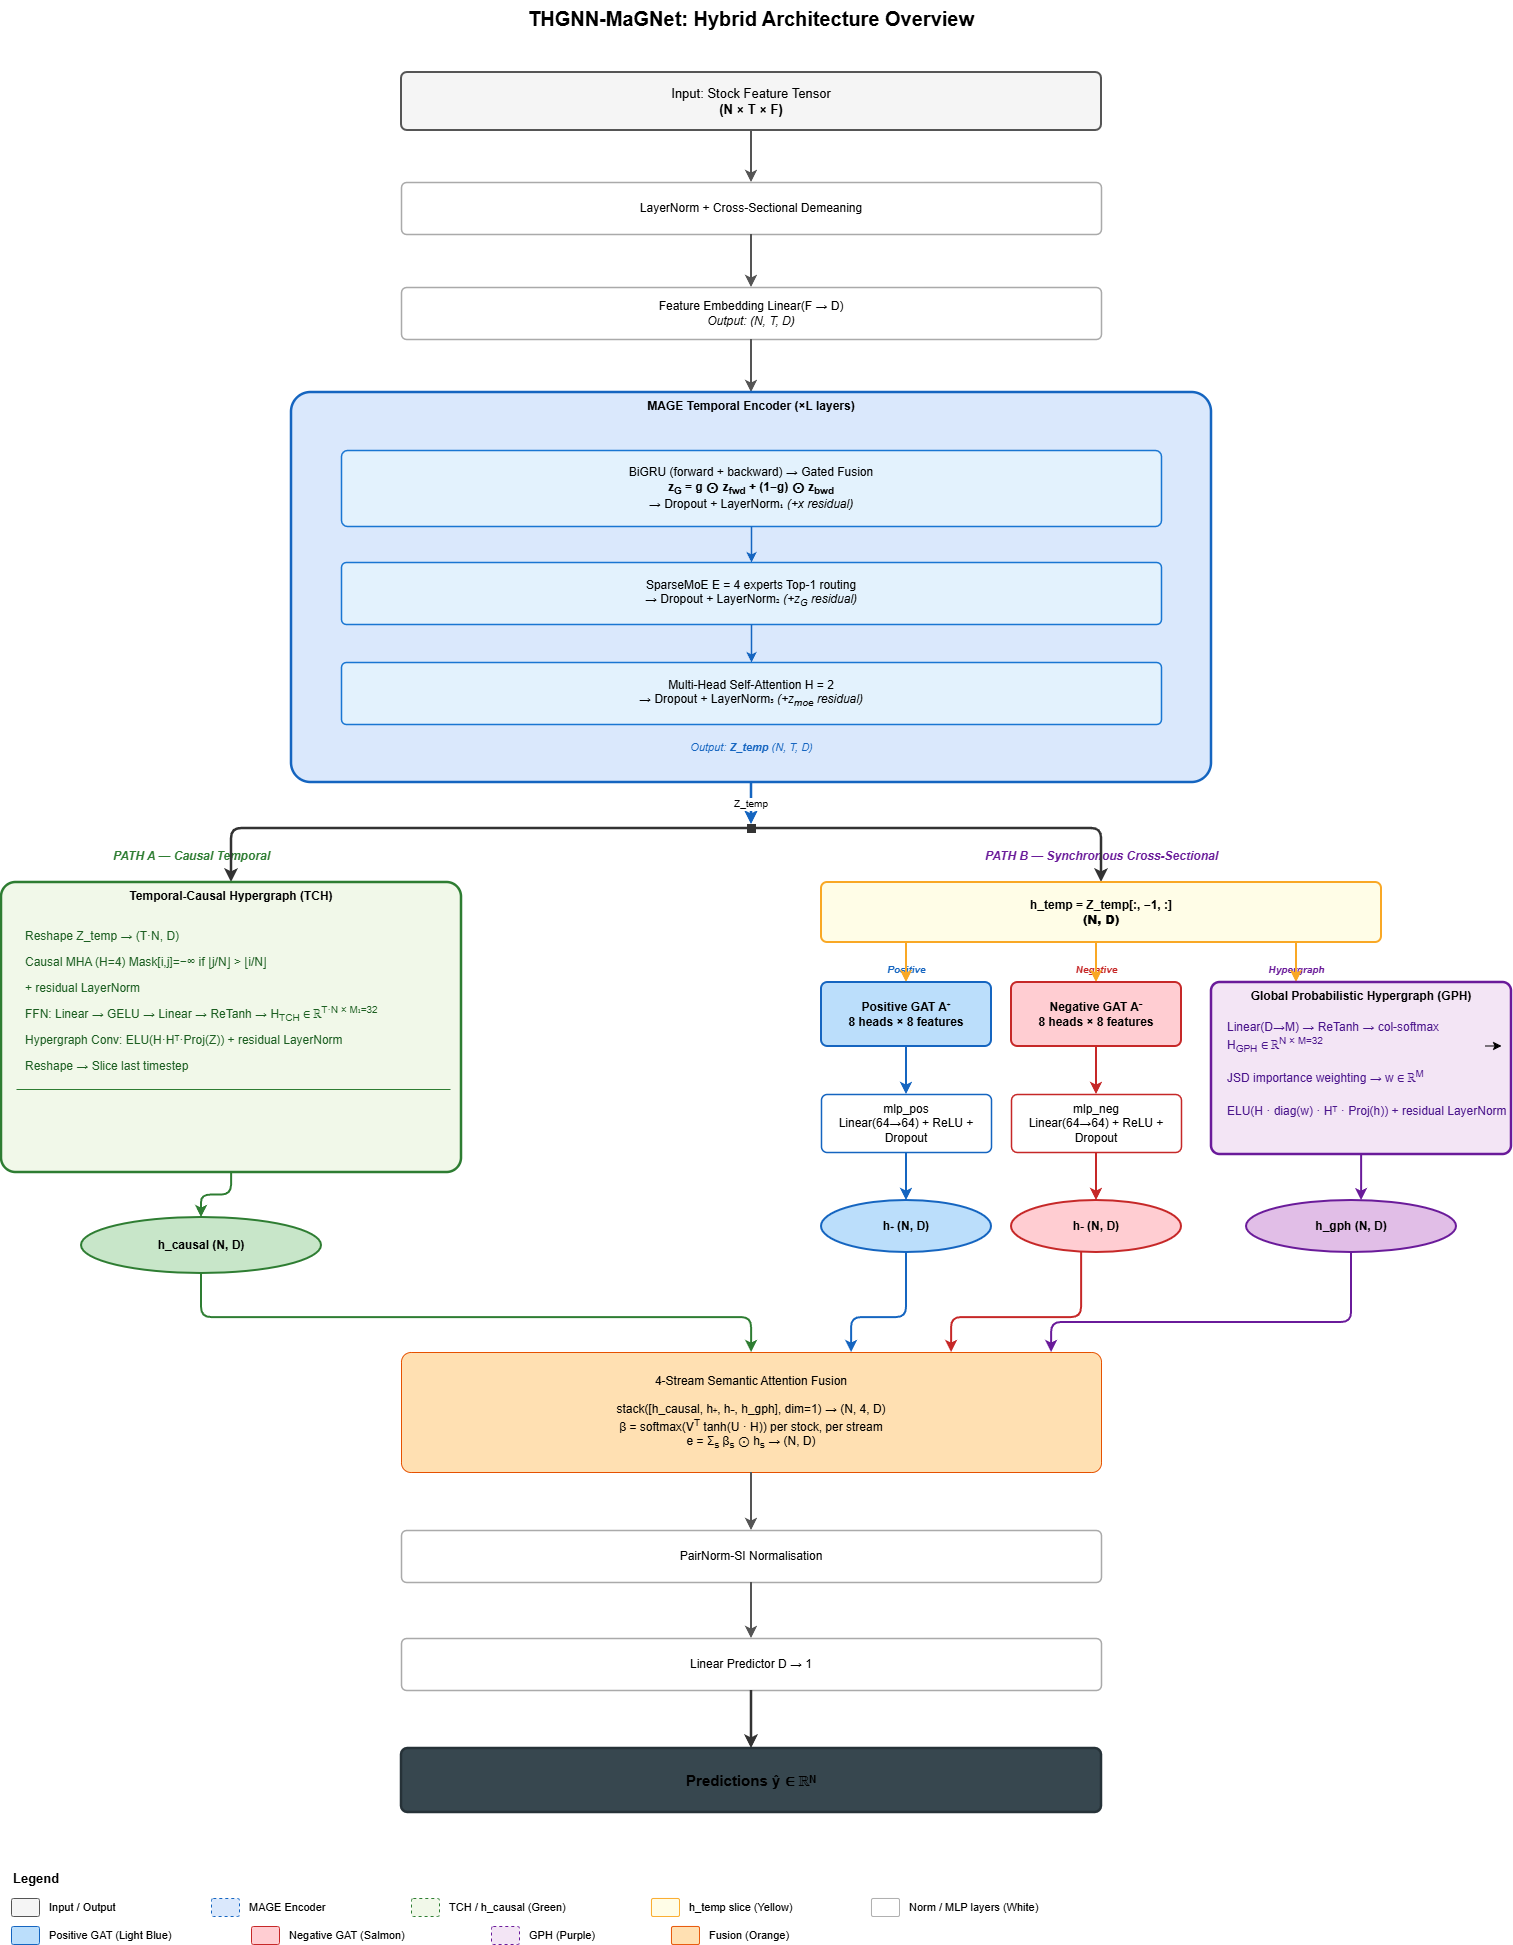
\includegraphics[width=0.95\textwidth]{figures/hybrid_architecture.png}
\caption{Overall architecture of the proposed THGNN-MaGNet model. The input feature tensor passes through feature embedding and a MAGE temporal encoder, then splits into Path~A (full sequence $\to$ TCH) and Path~B (final timestep $\to$ Pos/Neg GAT and GPH). Four representations are fused by 4-stream semantic attention before the prediction head.}
\label{fig:hybrid_arch}
\end{figure}

\section{Base Model: Temporal and Heterogeneous GNN}
\label{sec:base_thgnn}

The baseline model reimplements the THGNN architecture~\cite{xiang2022thgnn} on the NIFTY~500 universe and serves as the controlled reference for evaluating the hybrid extension (Figure~\ref{fig:base_thgnn}).

\begin{figure}[htbp]
\centering
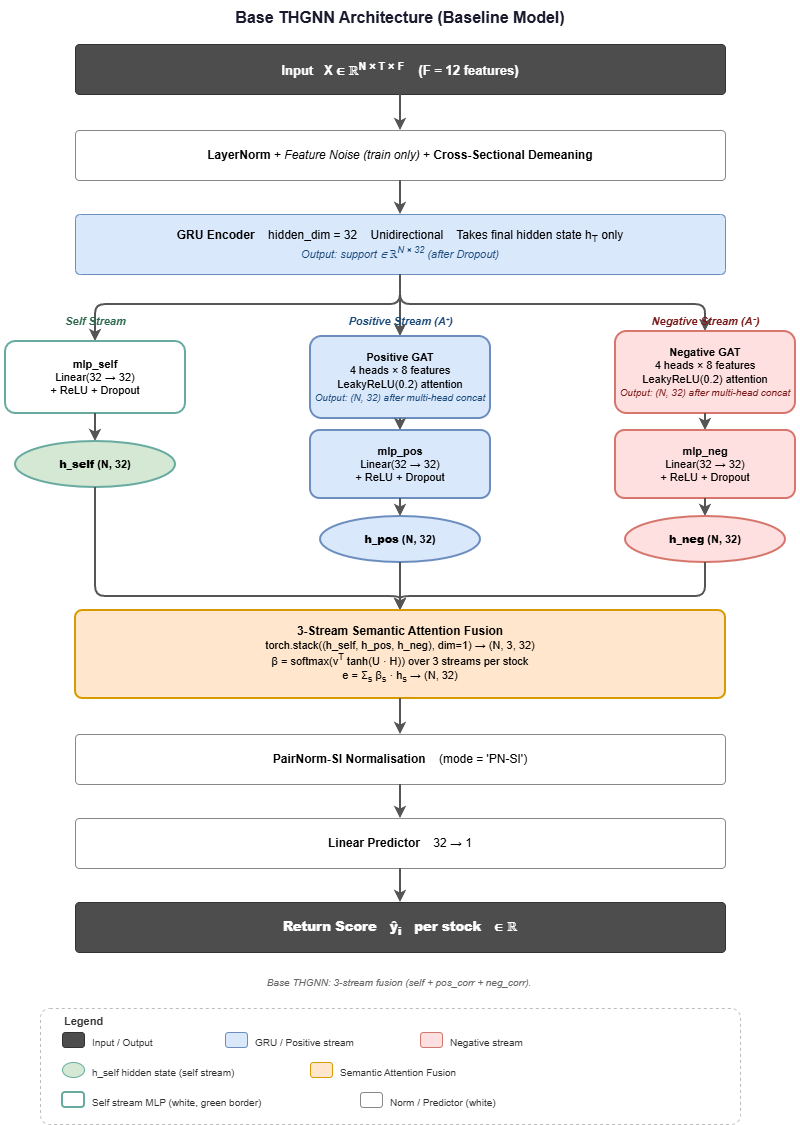
\includegraphics[width=0.70\textwidth]{figures/base_thgnn.png}
\caption{Base THGNN architecture. A unidirectional GRU encoder produces per-stock hidden states. Three streams (self, positive GAT, negative GAT) are fused by semantic attention before PairNorm and prediction.}
\label{fig:base_thgnn}
\end{figure}

In this reimplementation, the Transformer temporal encoder of the original THGNN is replaced by a GRU for computational efficiency on the 6\,GB GPU constraint; all other components (dynamic heterogeneous graph construction, positive/negative GAT streams, semantic attention fusion) follow the original design. A unidirectional GRU with hidden dimension $d_h = 128$ processes each stock's demeaned feature sequence, producing $\mathbf{z}_i = \mathbf{h}_T \in \mathbb{R}^{d_h}$. The standard GRU gating equations are:
\begin{align}
\mathbf{r}_t &= \sigma(\mathbf{W}_r \mathbf{x}_t + \mathbf{U}_r \mathbf{h}_{t-1}), \quad
\mathbf{u}_t = \sigma(\mathbf{W}_u \mathbf{x}_t + \mathbf{U}_u \mathbf{h}_{t-1}) \\
\tilde{\mathbf{h}}_t &= \tanh(\mathbf{W}_h \mathbf{x}_t + \mathbf{U}_h(\mathbf{r}_t \odot \mathbf{h}_{t-1})), \quad
\mathbf{h}_t = (1-\mathbf{u}_t)\odot\mathbf{h}_{t-1} + \mathbf{u}_t\odot\tilde{\mathbf{h}}_t
\end{align}

Three streams are computed from $\mathbf{z}_i$: a self-stream $\mathbf{h}^{\text{self}}_i = \text{ReLU}(\mathbf{W}_s\mathbf{z}_i)$, and two GAT streams over $\mathbf{A}^{+}$ and $\mathbf{A}^{-}$ with $H_{\text{gat}} = 4$ heads and $d_k = 8$ features per head. The per-head attention coefficient is:
\begin{equation}
\alpha^{h}_{ij} = \frac{
  \exp\!\bigl(\text{LReLU}_{0.2}\bigl(\mathbf{a}_h^{\top}[\mathbf{W}_h\mathbf{h}_i \| \mathbf{W}_h\mathbf{h}_j]\bigr)\bigr)
}{
  \sum_{k \in \mathcal{N}_i}\exp\!\bigl(\text{LReLU}_{0.2}\bigl(\mathbf{a}_h^{\top}[\mathbf{W}_h\mathbf{h}_i \| \mathbf{W}_h\mathbf{h}_k]\bigr)\bigr)
}
\end{equation}
A 3-stream semantic attention module assigns per-stock weights
\begin{equation}
\boldsymbol{\beta}_i = \text{softmax}\!\bigl(\mathbf{v}^{\top}\tanh(\mathbf{U}[\mathbf{h}^{\text{self}};\mathbf{h}^{+};\mathbf{h}^{-}])\bigr),
\end{equation}
producing fused embedding $\mathbf{e}_i = \sum_s \beta^s_i \mathbf{h}^s_i$. PairNorm-SI normalisation and a linear head yield the scalar return prediction.

\section{Hybrid Architecture: THGNN-MaGNet}
\label{sec:prop_hybrid}

\subsection{Input Processing}
Raw features are layer-normalised and cross-sectionally demeaned. A shared linear embedding projects from $F=12$ to $D=64$:
\begin{equation}
\mathbf{Z}^{(0)} = \tilde{\mathbf{X}}\mathbf{W}_{\text{emb}} \in \mathbb{R}^{N \times T \times D}
\end{equation}

\subsection{MAGE Temporal Encoder}

The MAGE block (Figure~\ref{fig:mage_block}; adapted from MaGNet~\cite{tan2025magnet} with the bidirectional Mamba layer replaced by a bidirectional GRU to accommodate the 6~GB GPU constraint, while retaining the SparseMoE and multi-head self-attention sub-layers) processes $\mathbf{Z}^{(0)}$ through three sequentially stacked sub-layers with residual connections and LayerNorm, producing $\mathbf{Z}_{\text{temp}} \in \mathbb{R}^{N \times T \times D}$.

\begin{figure}[htbp]
\centering
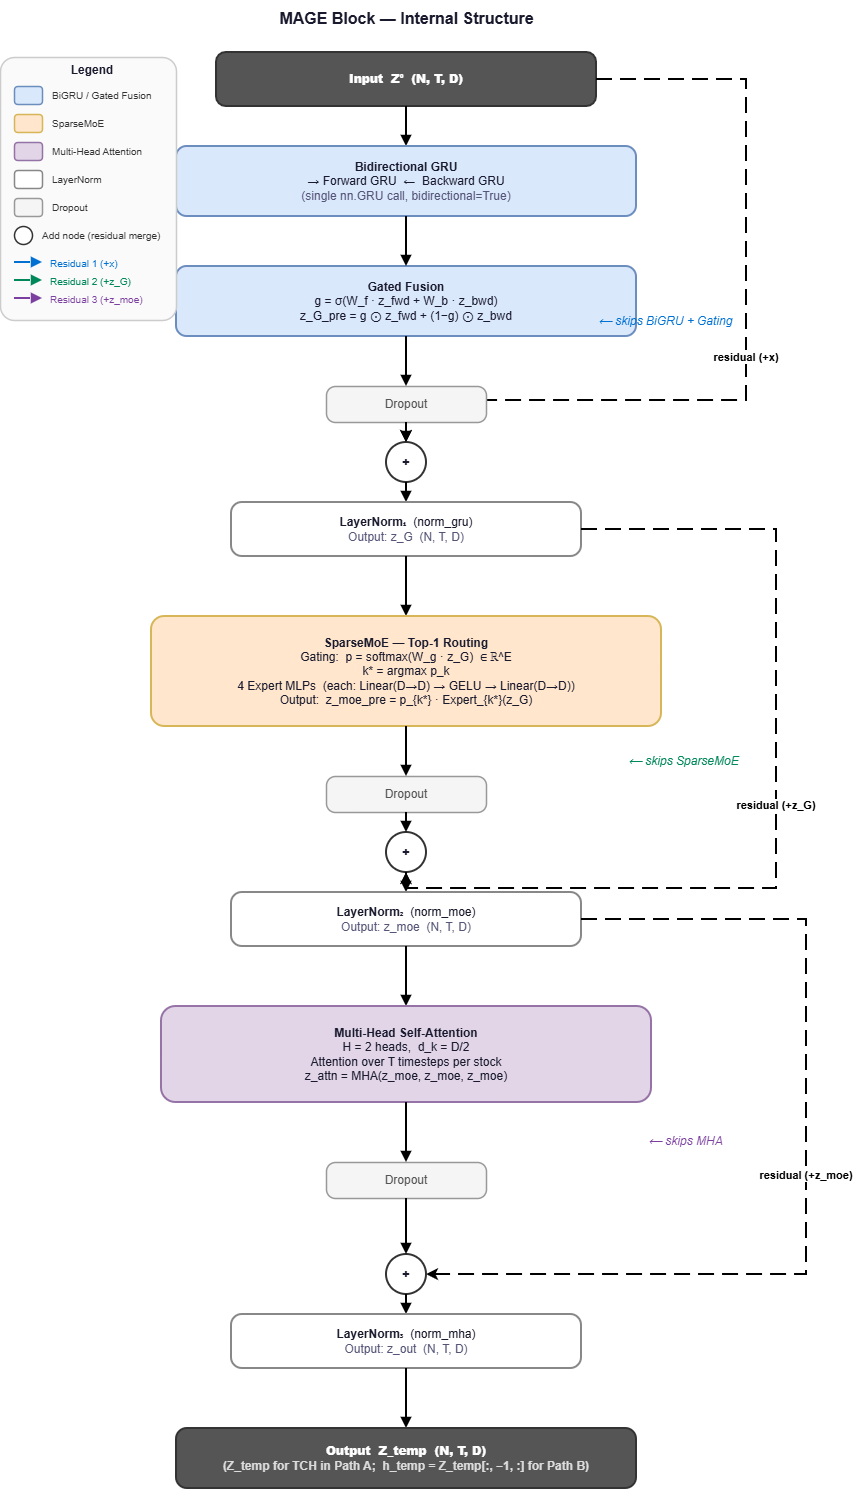
\includegraphics[width=0.75\textwidth]{figures/mage_block.png}
\caption{Internal structure of the MAGE block. Bidirectional GRU outputs are adaptively gated, routed to a Sparse Mixture-of-Experts (top-1, $E=4$), and contextualised by multi-head self-attention. Each sub-layer uses LayerNorm and a residual connection.}
\label{fig:mage_block}
\end{figure}

\paragraph{Bidirectional GRU with Gated Fusion.}
\begin{equation}
\mathbf{z}^{\text{fwd}} = \overrightarrow{\text{GRU}}(\mathbf{Z}^{(0)}), \quad \mathbf{z}^{\text{bwd}} = \overleftarrow{\text{GRU}}(\mathbf{Z}^{(0)})
\end{equation}
\begin{equation}
\mathbf{g} = \sigma(\mathbf{W}_f\mathbf{z}^{\text{fwd}} + \mathbf{W}_b\mathbf{z}^{\text{bwd}}), \quad
\mathbf{z}^{\text{gru}} = \mathbf{g}\odot\mathbf{z}^{\text{fwd}} + (1-\mathbf{g})\odot\mathbf{z}^{\text{bwd}}
\end{equation}

\paragraph{Sparse Mixture-of-Experts.}
$E = 4$ expert MLPs each have the form $\text{Expert}_k(\mathbf{z}) = \mathbf{W}^{(2)}_k\,\text{GELU}(\mathbf{W}^{(1)}_k\mathbf{z})$. Top-1 routing is applied:
\begin{equation}
\mathbf{p} = \text{softmax}(\mathbf{W}_g\mathbf{z}^{\text{gru}}), \quad k^* = \arg\max_k p_k, \quad
\mathbf{z}^{\text{moe}} = p_{k^*}\cdot\text{Expert}_{k^*}(\mathbf{z}^{\text{gru}})
\end{equation}
The routing probability $p_{k^*}$ scales the selected expert's output, preserving gradient flow through the gating network. Different experts specialise in different market regimes (trending vs.\ mean-reverting), enabling adaptive temporal feature extraction without explicit regime labels.

\paragraph{Multi-Head Self-Attention.}
\begin{equation}
\mathbf{Z}_{\text{temp}} = \text{LayerNorm}\!\left(\mathbf{z}^{\text{moe}} + \text{MHA}(\mathbf{z}^{\text{moe}},\mathbf{z}^{\text{moe}},\mathbf{z}^{\text{moe}};\;H_{\text{mage}}=2)\right)
\end{equation}

\subsection{Temporal-Causal Hypergraph (TCH)}

The TCH (Figure~\ref{fig:dual_hypergraph}, left) captures asynchronous inter-stock lead-lag dependencies by operating over a spatiotemporal node set of size $T \cdot N$.

\paragraph{Reshape and Causal Attention.}
$\mathbf{Z}_{\text{temp}}$ is reshaped to $\mathbf{Z}' \in \mathbb{R}^{(TN)\times D}$. Causally masked multi-head attention ($H_{\text{tch}}=4$) is applied with a block-triangular mask:
\begin{equation}
\mathbf{Z}_{\text{attn}} = \text{MHA}(\mathbf{Z}';\;\text{Mask}_{ij}=-\infty \text{ if } \lfloor j/N \rfloor > \lfloor i/N \rfloor)
\end{equation}
This ensures that node $(t,s)$ cannot attend to nodes $(t',s')$ where $t' > t$ (future keys are masked), preserving strict causal structure.

\paragraph{Learned Hyperedge Incidence (end-to-end, addresses Gap~1).}
\begin{equation}
\mathbf{H}_{\text{TCH}} = \text{ReTanh}\!\left(\mathbf{W}_{h2}\,\text{GELU}(\mathbf{W}_{h1}\mathbf{Z}_{\text{attn}})\right) \in \mathbb{R}^{(TN)\times M_1}
\end{equation}
where $\text{ReTanh}(x)=\max(0,\tanh(x))$ produces sparse, bounded membership values, and $M_1 = 32$. Because $\mathbf{H}_{\text{TCH}}$ is the output of a learned network trained jointly with the prediction loss, the hyperedge topology is optimised end-to-end. Combined with the causal attention mask, this directly addresses the causal aspect of Gap~1.

\paragraph{Hypergraph Convolution.}
\begin{equation}
\mathbf{Z}_{\text{conv}} = \text{ELU}\!\left(\mathbf{H}_{\text{TCH}}\cdot\left(\mathbf{H}_{\text{TCH}}^{\top}\cdot\mathbf{Z}'\mathbf{W}_{\text{proj}}\right)\right) + \mathbf{Z}_{\text{attn}}
\end{equation}
This implements the hypergraph Laplacian propagation $\boldsymbol{\Delta}=\mathbf{H}\mathbf{W}_e\mathbf{H}^{\top}$ with uniform edge weights. The causal representation is extracted from the final timestep: $\mathbf{h}_{\text{causal}} = \mathbf{Z}_{\text{conv}}[:,T{-}1,:] \in \mathbb{R}^{N \times D}$.

\subsection{Global Probabilistic Hypergraph (GPH)}

The GPH (Figure~\ref{fig:dual_hypergraph}, right) models market-wide thematic groupings using soft learned membership and JSD-based importance weighting.

\paragraph{Soft Membership.}
\begin{equation}
\mathbf{H}_{\text{GPH}} = \text{softmax}_{\text{col}}\!\left(\text{ReTanh}(\mathbf{W}_{\text{gph}}\,\mathbf{h}_{\text{temp}})\right) \in \mathbb{R}^{N \times M}
\end{equation}
Column-wise softmax ensures each of the $M=32$ hyperedges defines a valid distribution over the $N$ stocks.

\paragraph{JSD Importance Weighting.}
Hyperedge importance is measured by distinctiveness from other hyperedges:
\begin{equation}
\text{JSD}_{mm'} = \frac{1}{2}\text{KL}\!\left(\mathbf{H}_{:,m}\,\|\,\mathbf{M}_{mm'}\right) + \frac{1}{2}\text{KL}\!\left(\mathbf{H}_{:,m'}\,\|\,\mathbf{M}_{mm'}\right), \quad
\mathbf{M}_{mm'} = \tfrac{1}{2}(\mathbf{H}_{:,m}+\mathbf{H}_{:,m'})
\end{equation}
\begin{equation}
w_m = \text{softmax}\!\left(\text{zscore}\!\left(\textstyle\tfrac{1}{M}\sum_{m'\neq m}\text{JSD}_{mm'}\right)\right)
\end{equation}

\paragraph{Hypergraph Convolution.}
\begin{equation}
\mathbf{h}_{\text{gph}} = \text{ELU}\!\left(\mathbf{H}_{\text{GPH}}\cdot\left(\mathbf{w}\otimes\left(\mathbf{H}_{\text{GPH}}^{\top}\cdot\mathbf{h}_{\text{temp}}\mathbf{W}_p\right)\right)\right) + \mathbf{h}_{\text{temp}}
\end{equation}

\begin{figure}[htbp]
\centering
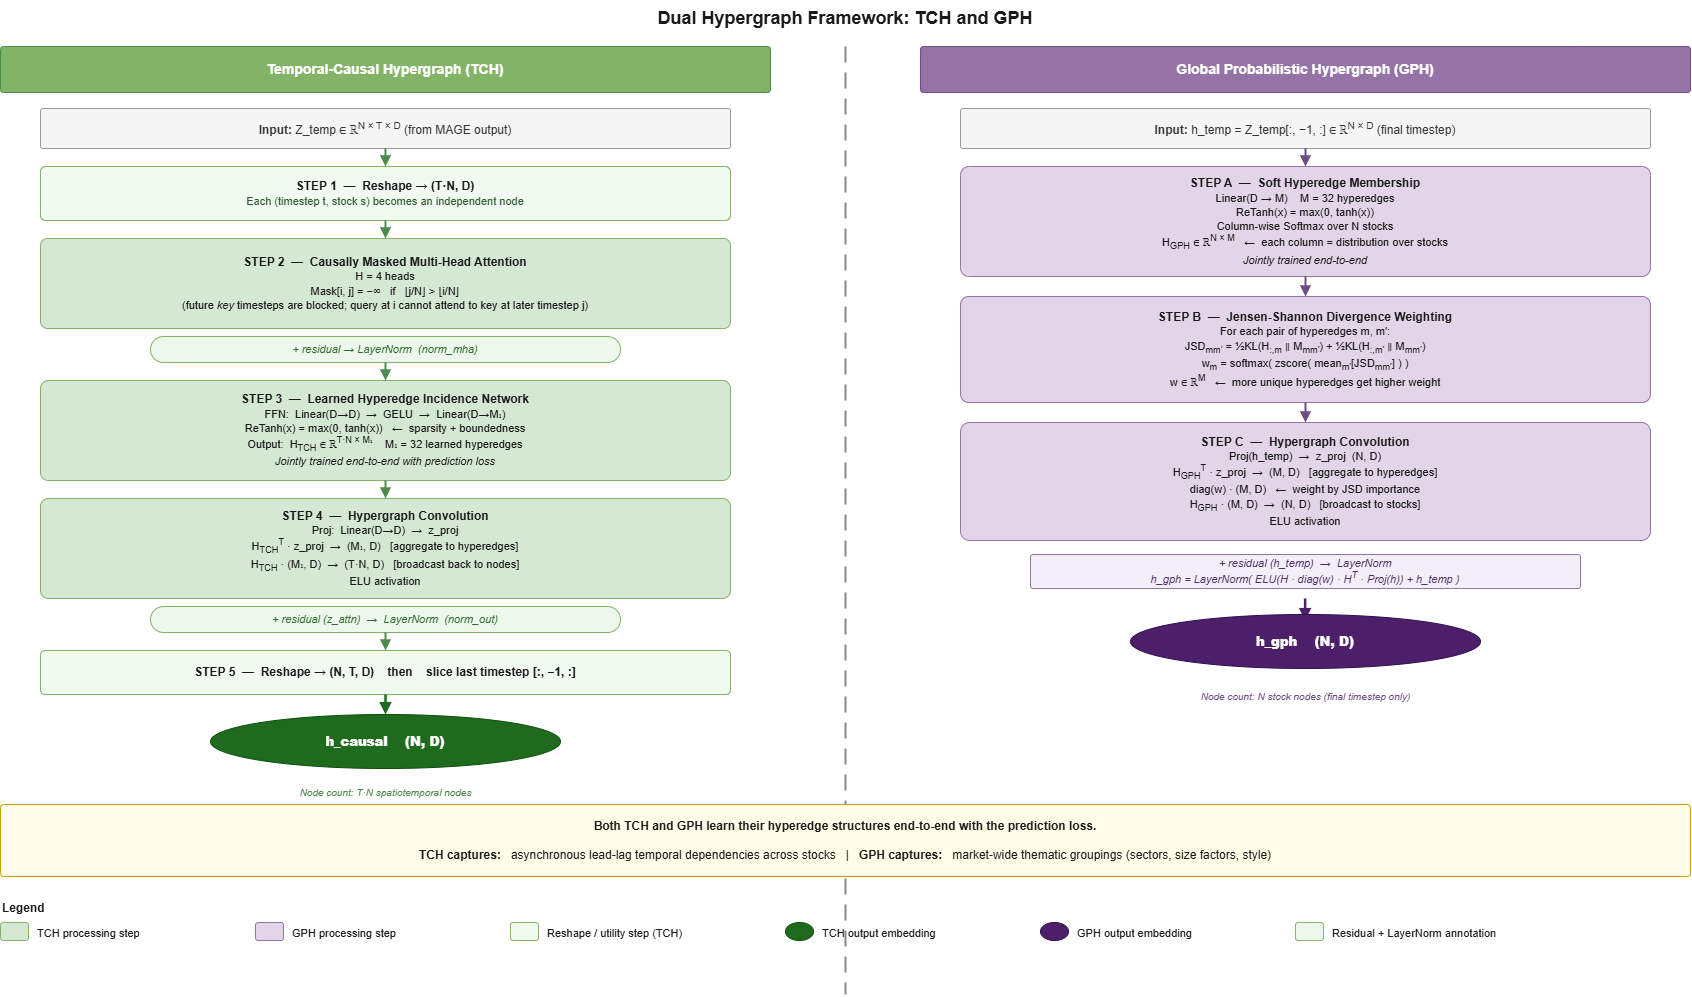
\includegraphics[width=\textwidth]{figures/dual_hypergraph.png}
\caption{\textbf{Left:} Temporal-Causal Hypergraph (TCH). The MAGE output is reshaped to $T{\cdot}N$ spatiotemporal nodes; causally masked attention and a learned FFN produce $M_1{=}32$ causal hyperedges via ReTanh activation. \textbf{Right:} Global Probabilistic Hypergraph (GPH). Soft column-normalised membership and JSD-weighted convolution capture thematic market groupings. Both incidence matrices are trained end-to-end.}
\label{fig:dual_hypergraph}
\end{figure}

\subsection{Cross-Sectional Streams: Positive and Negative GAT}

From $\mathbf{h}_{\text{temp}}$, two typed graph attention networks model pairwise heterogeneous correlation relationships, following the THGNN design. Each GAT uses $H_{\text{gat}}=8$ heads with $d_k=8$ per head (output dim 64), with LeakyReLU$(0.2)$ attention and an MLP projection back to $D=64$. The pairwise correlation edges provide an explicit inductive bias that complements the soft learned hyperedges.

\subsection{4-Stream Semantic Attention Fusion}

The four representations $\mathbf{H} = [\mathbf{h}_{\text{causal}};\,\mathbf{h}_{+};\,\mathbf{h}_{-};\,\mathbf{h}_{\text{gph}}] \in \mathbb{R}^{N \times 4 \times D}$ are fused via learned per-stock stream weights:
\begin{equation}
\mathbf{w} = \mathbf{V}^{\top}\tanh(\mathbf{U}\mathbf{H}) \in \mathbb{R}^{N \times 4}, \quad
\boldsymbol{\beta} = \text{softmax}(\mathbf{w}) \in \mathbb{R}^{N \times 4}
\end{equation}
\begin{equation}
\mathbf{e} = \sum_{s=1}^{4}\beta_{:,s}\odot\mathbf{H}_{:,s,:} \in \mathbb{R}^{N \times D}
\end{equation}
Each stock adaptively weights its causal temporal context, positive-correlation neighbourhood, negative-correlation neighbourhood, and global thematic group.

\subsection{Prediction Head}

PairNorm-SI prevents over-smoothing by instance-normalising the fused embeddings:
\begin{equation}
\hat{\mathbf{e}}_i = \frac{\mathbf{e}_i - \bar{\mathbf{e}}}{\sqrt{\varepsilon + \|\mathbf{e}_i - \bar{\mathbf{e}}\|^2}}, \quad \bar{\mathbf{e}} = \tfrac{1}{N}\textstyle\sum_i\mathbf{e}_i
\end{equation}
The final prediction is $\hat{\mathbf{y}} = \hat{\mathbf{e}}\mathbf{W}_{\text{pred}} \in \mathbb{R}^N$.

\section{Training Objective}
\label{sec:training}

The composite loss combines three terms:
\begin{equation}
\mathcal{L} = \lambda_{\text{mse}}\mathcal{L}_{\text{mse}} + \tilde{\lambda}_{\text{ic}}(e)\,\mathcal{L}_{\text{ic}} + \lambda_{\text{disp}}\mathcal{L}_{\text{disp}}
\end{equation}
with weights $\lambda_{\text{mse}}=0.4$, $\lambda_{\text{ic}}=0.8$, $\lambda_{\text{disp}}=0.1$ for the Hybrid BiGRU model; the Mamba--MoE variant uses $\lambda_{\text{mse}}=0.6$, $\lambda_{\text{ic}}=0.6$, $\lambda_{\text{disp}}=0.1$ (see Table~\ref{tab:hyperparams}).

\paragraph{MSE Component.}
\begin{equation}
\mathcal{L}_{\text{mse}} = \frac{1}{N\sigma_r^2}\sum_{i=1}^{N}\!\left(\hat{y}^{\text{cs}}_i - y^{\text{cs}}_i\right)^2, \quad \sigma_r = 0.02
\end{equation}
where $\hat{y}^{\text{cs}} = \hat{\mathbf{y}}-\bar{\hat{y}}$ and $y^{\text{cs}}=\mathbf{y}-\bar{y}$ are cross-sectionally demeaned, and $\sigma_r^2$ normalises to unit-free magnitude.

\paragraph{Differentiable Spearman IC Component.}
Standard Spearman rank correlation is non-differentiable. A soft rank is computed via pairwise sigmoid comparisons with annealing temperature:
\begin{equation}
r^{\text{soft}}_i(\hat{\mathbf{y}}) = \sum_{j=1}^{N}\sigma\!\left(\frac{\hat{y}_i - \hat{y}_j}{\tau_e}\right), \quad \tau_e = \max(0.02,\; 0.2\cdot 0.95^e)
\end{equation}
The temperature $\tau_e$ anneals from 0.20 (soft, exploration-biased) to 0.02 (hard, exploitation-biased) over training. The IC is estimated between soft-ranked predictions and soft-ranked targets (targets detached):
\begin{equation}
\text{IC}_{\text{soft}} = \frac{(r^{\text{soft}}(\hat{\mathbf{y}})-\bar{r}^{\text{soft}})^{\top}(r^{\text{soft}}(\mathbf{y})-\bar{r}^{y,\text{soft}})}{\|r^{\text{soft}}(\hat{\mathbf{y}})-\bar{r}^{\text{soft}}\|\cdot\|r^{\text{soft}}(\mathbf{y})-\bar{r}^{y,\text{soft}}\|+\varepsilon}, \quad
\mathcal{L}_{\text{ic}} = 1 - \text{IC}_{\text{soft}}
\end{equation}
The IC weight is linearly warmed up over $E_{\text{warmup}}=5$ epochs: $\tilde{\lambda}_{\text{ic}}(e)=\lambda_{\text{ic}}\cdot\min(1,e/E_{\text{warmup}})$, preventing the ranking loss from dominating before the model has learned useful price representations.

\paragraph{Dispersion Component.}
\begin{equation}
\mathcal{L}_{\text{disp}} = \text{ReLU}(\kappa_{\min}-\kappa) + \text{ReLU}(\kappa-\kappa_{\max}), \quad \kappa = \sigma_{\hat{y}}/\sigma_y
\end{equation}
with $\kappa_{\min}=0.3$ and $\kappa_{\max}=3.0$ (distinct from Spearman $\rho$ used elsewhere). This penalises prediction collapse ($\kappa\to 0$) and excessive spread ($\kappa\gg 1$).

\paragraph{Optimisation.}
AdamW ($\text{lr}=2\times10^{-4}$, weight decay $=10^{-4}$) is used with gradient clipping (max norm 1.0) and a three-phase learning rate schedule: linear warmup for 5 epochs, flat plateau for 20 epochs, then cosine decay to $10^{-5}$.

Table~\ref{tab:complexity} compares the asymptotic complexity of the three model variants per training step ($N$: stocks, $T$: timesteps, $D$: embedding dim, $M_1,M$: hyperedge counts, $S$: SSM state dim).

\begin{table}[htbp]
\centering
\small
\caption{Asymptotic time complexity per training step for each model variant.}
\label{tab:complexity}
\resizebox{\linewidth}{!}{%
\begin{tabular}{lll}
\toprule
\textbf{Model} & \textbf{Temporal Encoder} & \textbf{Relational Module} \\
\midrule
THGNN (baseline)    & $O(NTd_hF)$ GRU               & $O(N^2d_h)$ GAT \\
Hybrid (BiGRU+MoE)  & $O(NTD^2)$ BiGRU + MoE + MHA  & $O((TN)^2D)$ TCH-MHA $+$ $O(TNM_1D)$ TCH-HG $+$ $O(N^2D)$ GAT $+$ $O(NMD)$ GPH \\
Hybrid (Mamba+MoE)  & $O(NTDS)$ SSM scan             & Same relational modules \\
\bottomrule
\end{tabular}}
\end{table}

The TCH relational module has two cost components: the causal multi-head attention over $TN$ (time, stock) node pairs, which is $O((TN)^2D)$; and the hypergraph convolution via $M_1$ hyperedges, which is the cheaper $O(TNM_1D)$ term. With $T=20$, $N=353$, $D=64$, $M_1=32$, the causal MHA produces an attention matrix of size $TN \times TN = 7060 \times 7060 \approx 50$M elements per head ($\approx$200~MB in float32 per head, $\approx$800~MB total across $H_{\text{tch}}{=}4$ heads), which is tractable on a 6~GB GPU alongside the remaining activations. The Mamba variant reduces the temporal encoder from quadratic (BiGRU MHA) to near-linear ($O(NTDS)$ selective scan) in sequence length, at the cost of requiring a CUDA-compatible GPU for the optimised parallel scan kernel.

\section{Multi-Agent Decision Pipeline}
\label{sec:multiagent}

The trained GNN model serves as the core inference engine within a six-agent LangGraph pipeline (Figure~\ref{fig:multiagent}) that transforms raw market data into a structured investment recommendation, integrating GNN-based quantitative predictions with real-time news sentiment, macroeconomic regime context, and systematic risk profiling.

\begin{figure}[htbp]
\centering
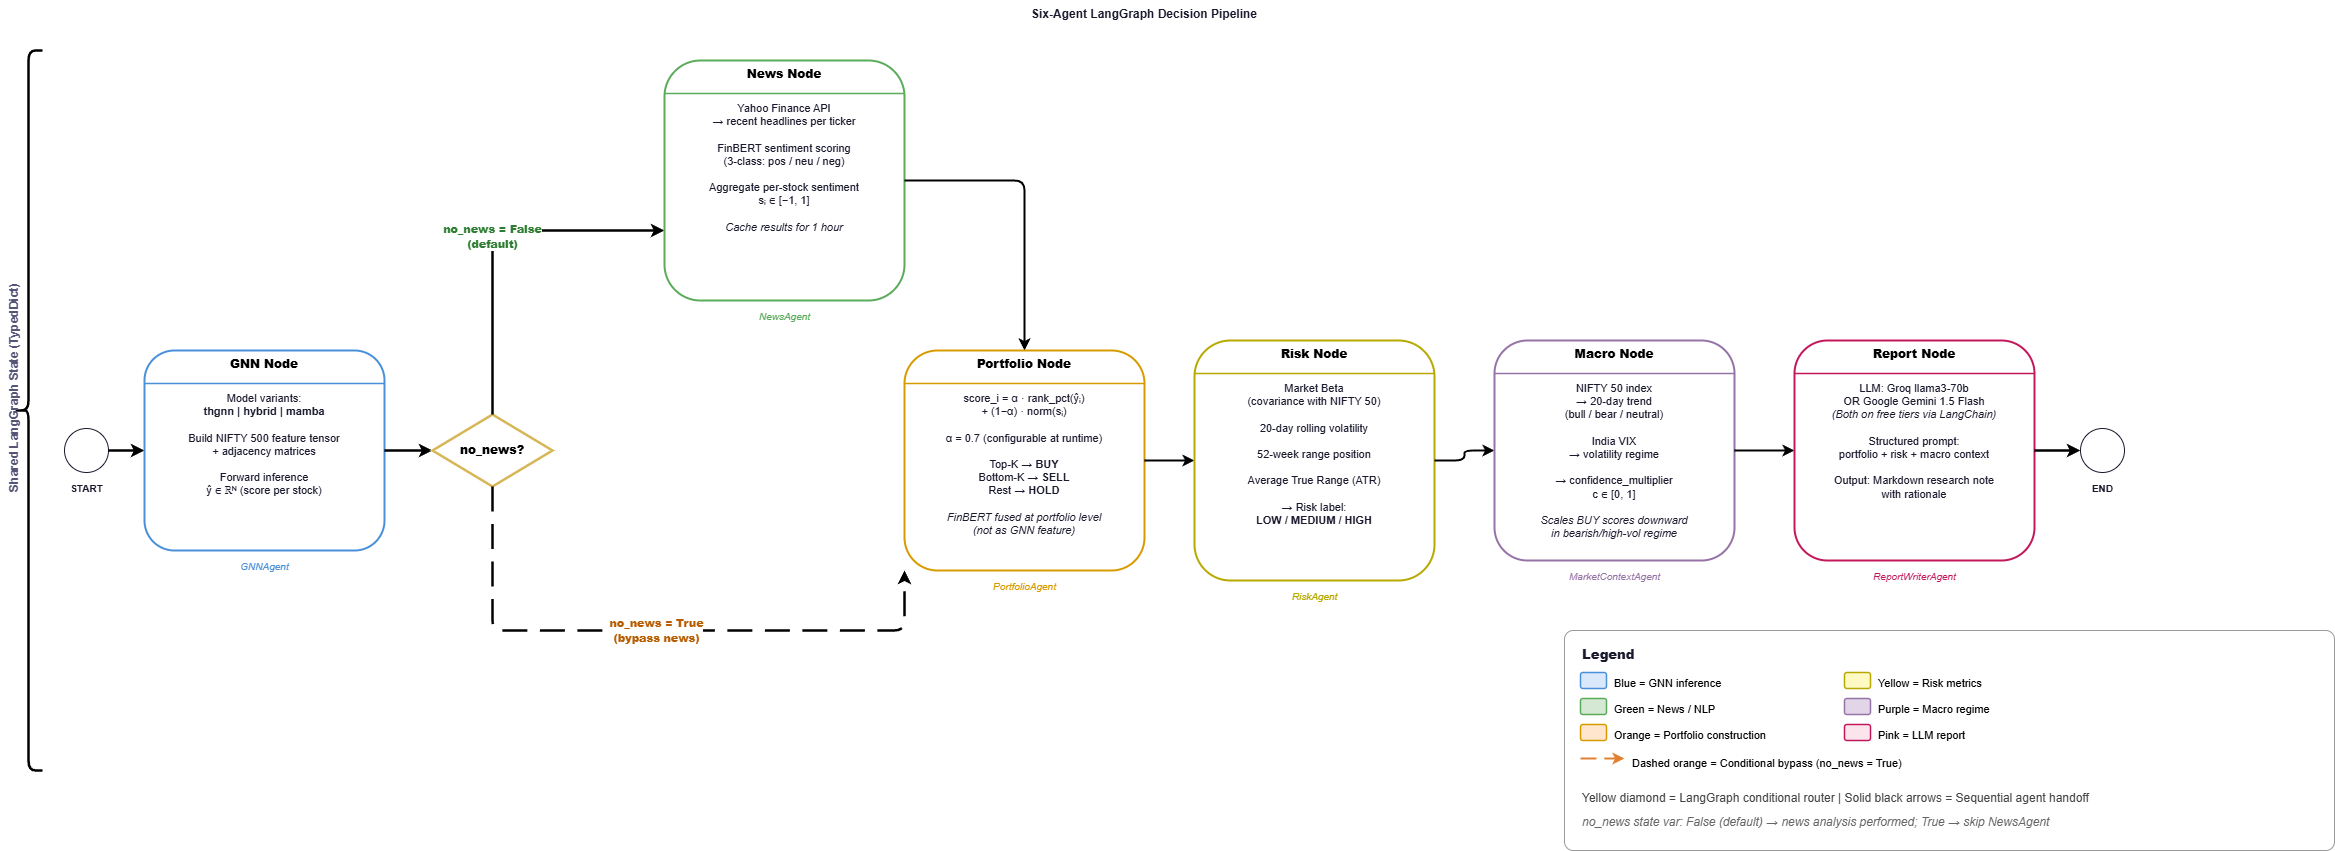
\includegraphics[width=\textwidth]{figures/multiagent_pipeline.png}
\caption{Six-agent LangGraph pipeline for end-to-end financial decision support. A conditional edge from the GNN Node allows the news step to be bypassed for faster inference. All six agents share a typed state dictionary propagated through the graph.}
\label{fig:multiagent}
\end{figure}

\begin{enumerate}
    \item \textbf{GNN Node:} Loads the trained checkpoint for the selected model variant (\texttt{thgnn}, \texttt{hybrid}, or \texttt{mamba}), constructs the NIFTY~500 feature tensor and adjacency matrices for the target trading day, and runs forward inference to produce raw score vector $\hat{\mathbf{y}} \in \mathbb{R}^N$.

    \item \textbf{News Node:} Fetches recent headlines via the Yahoo Finance API and scores each headline with FinBERT~\cite{araci2019finbert}, a BERT model pre-trained on financial text. Per-stock sentiment scores $s_i \in [-1,1]$ are aggregated from the three-class (positive/neutral/negative) probability outputs across all headlines within a 24-hour window and cached for one hour.

    \item \textbf{Portfolio Node:} Fuses GNN and sentiment signals into a final allocation score:
    \begin{equation}
    \text{score}_i = \alpha\cdot\text{rank}_{\text{pct}}(\hat{y}_i) + (1-\alpha)\cdot\text{norm}(s_i)
    \end{equation}
    where $\alpha \in [0,1]$ is a tunable inference-time parameter (default $\alpha=0.7$; set to $\alpha=0.60$ in the live demonstration of Section~\ref{sec:pipeline_demo}). The top-$K$ stocks are designated BUY and the bottom-$K$ are SELL. Crucially, FinBERT sentiment is fused at the \emph{portfolio level} rather than as a GNN input feature, preserving the model's price-based relational learning while allowing $\alpha$ to be adjusted at inference time without retraining.

    \item \textbf{Risk Node:} Computes four risk metrics from 90-day OHLCV history for each BUY/SELL candidate: market beta (covariance with NIFTY~50), 20-day rolling volatility, 52-week range position, and Average True Range (ATR). Each stock receives a composite risk label (LOW/MEDIUM/HIGH).

    \item \textbf{Macro Node:} Assesses the macro regime from the NIFTY~50 20-day trend and India VIX level, producing a confidence multiplier $c\in[0,1]$ that scales BUY scores downward in bearish or high-volatility regimes---providing systematic regime-aware position sizing.

    \item \textbf{Report Node:} Invokes Google \texttt{gemma-4-31b} via LangChain with a structured prompt encoding the portfolio table, risk labels, and macro context. The LLM generates a Markdown-formatted research note summarising the allocation rationale, sector exposures, and key risks.
\end{enumerate}

\chapter{Results}
\label{ch:Results}

\section{Experimental Setup}

All experiments use a three-way temporal split designed to prevent information leakage from the evaluation period into model selection:

\begin{itemize}
    \item \textbf{Training set:} 1~January~2015 -- 31~December~2022 (approximately 1,957 trading days). Used exclusively for gradient updates.
    \item \textbf{Validation set:} 1~January~2023 -- 31~December~2023 (approximately 252 trading days). Used for early stopping and checkpoint selection (the epoch with the highest validation rank-IC is retained). The model never receives gradient updates from this split.
    \item \textbf{Holdout set:} 1~January~2024 -- 15~May~2026 (approximately 583 trading days). Evaluated only once, against the best checkpoint. All reported IC, MSE, and directional accuracy figures are computed on this split.
\end{itemize}


\subsection{Stock Universe and Features}

The NIFTY~500 constituent list is filtered to retain stocks with at least 250 consecutive trading days of non-null OHLCV data, yielding a universe of 353 symbols traded on the National Stock Exchange (NSE). Per-stock daily feature vectors and cross-sectional demeaning follow Section~\ref{sec:problem} ($F=12$ signals, $T=20$ lookback). The prediction target is the cross-sectionally demeaned next-day return.

\subsection{Training Hyperparameters}

Table~\ref{tab:hyperparams} lists the key hyperparameters for each model variant as used in the best-checkpoint run.

\begin{table}[htbp]
\centering
\caption{Hyperparameters for best-checkpoint run of each model variant.}
\label{tab:hyperparams}
\begin{tabular}{lccc}
\toprule
\textbf{Hyperparameter} & \textbf{Base THGNN} & \textbf{Hybrid BiGRU} & \textbf{Mamba--MoE} \\
\midrule
Input features & 12 & 12 & 12 \\
Hidden / embed dim ($d_h$ / $D$) & 128 & 64 & 64 \\
GAT heads & 4 & 8 & 8 \\
MAGE layers & --- & 1 & 1 \\
MoE experts & --- & 4 & 4 \\
MHA heads & --- & 2 & 2 \\
Hyperedges (GPH / TCH) & --- & 32 / 32 & 32 / 32 \\
Learning rate (peak) & $1\times10^{-4}$ & $2\times10^{-4}$ & $1\times10^{-4}$ \\
Weight decay & $5\times10^{-5}$ & $1\times10^{-4}$ & $1\times10^{-4}$ \\
Dropout & 0.25 & 0.20 & 0.30 \\
MSE / IC / Disp weights & 0.7 / 0.5 / 0.6 & 0.4 / 0.8 / 0.1 & 0.6 / 0.6 / 0.1 \\
IC warmup (epochs) & 5 & 5 & 10 \\
\bottomrule
\end{tabular}
\end{table}

All models were trained on a single NVIDIA RTX~3050 6\,GB GPU (CUDA~12.4) with mixed-precision disabled. The Hybrid BiGRU model has 172,637 trainable parameters and takes approximately 160\,s per epoch; the Mamba--MoE takes approximately 200\,s per epoch; the Base THGNN takes approximately 23\,s per epoch owing to its simpler architecture.

\section{Quantitative Results}

Table~\ref{tab:main_results} presents the primary evaluation metrics at the checkpoint epoch selected by peak validation Information Coefficient (IC). The IC reported is the Spearman rank correlation (rank-IC) between predicted and realised next-day returns across all stocks on each test day, averaged over the test window. Mean-squared error (MSE) is computed on normalised return predictions. Directional accuracy (Dir-Acc) measures the fraction of stock-days on which the sign of the predicted return matches the sign of the realised return.

\begin{table}[htbp]
\centering
\caption{Holdout performance across all model variants (2024-01-01 -- 2026-05-15). Rank-IC is the Spearman rank correlation between predicted and realised next-day returns, averaged over all holdout trading days ($T_{\mathrm{holdout}}\approx583$). Approximate standard error: $\widehat{\mathrm{SE}} = \sqrt{1/(N_{\mathrm{stocks}}-2)}\,/\sqrt{T_{\mathrm{holdout}}} \approx 0.0534/\sqrt{583} \approx 0.0022$ (asymptotic Spearman SE for $N=353$ stocks per day, divided by $\sqrt{T_{\mathrm{holdout}}}$ under the assumption of i.i.d.\ daily IC observations). Best values in bold.}
\label{tab:main_results}
\resizebox{\linewidth}{!}{%
\begin{tabular}{lccccc}
\toprule
\textbf{Model} & \textbf{Best Epoch} & \textbf{Rank-IC} & \textbf{$\approx$SE} & \textbf{MSE} & \textbf{Dir-Acc (\%)} \\
\midrule
Base THGNN (GRU $+$ 3-stream GAT) & 2 & 0.0204 & 0.0022 & 1.3214 & 48.7 \\
Mamba--MoE (Mamba SSM $+$ MAGE $+$ Dual Hyp.) & 60 & 0.0343 & 0.0022 & 1.2560 & 50.8 \\
Hybrid BiGRU (BiGRU $+$ MAGE $+$ Dual Hyp.) & \textbf{65} & \textbf{0.0398} & 0.0023 & \textbf{1.1094} & 50.4 \\
\bottomrule
\end{tabular}}
\end{table}

The \textbf{Mamba--MoE} variant uses a Mamba selective state-space model~\cite{gu2024mamba} (with a pure-PyTorch fallback for environments without the \texttt{mamba-ssm} CUDA package) as the sequence mixer inside the MAGE block, replacing the bidirectional GRU used by the BiGRU variant. All other architectural components (SparseMoE, MHA, TCH, GPH, GAT streams) are identical between the two hybrid variants.

All three rank-IC estimates are statistically significant: the approximate $t$-statistics---computed as $\text{IC}/\widehat{\text{SE}}$ using the asymptotic Spearman SE formula---are $t \approx 9.3$ (Base THGNN), $t \approx 15.6$ (Mamba--MoE), and $t \approx 17.3$ (Hybrid BiGRU), all $p < 0.0001$ under a one-sided $t$-test against zero. The daily IC ACF (Figure~\ref{fig:ic_acf}) confirms no significant serial dependence at any lag 1--20 (95\% Bartlett CI), empirically validating the i.i.d.\ assumption and confirming the reported $t$-statistics are not materially inflated by autocorrelation.

\begin{figure}[htbp]
\centering
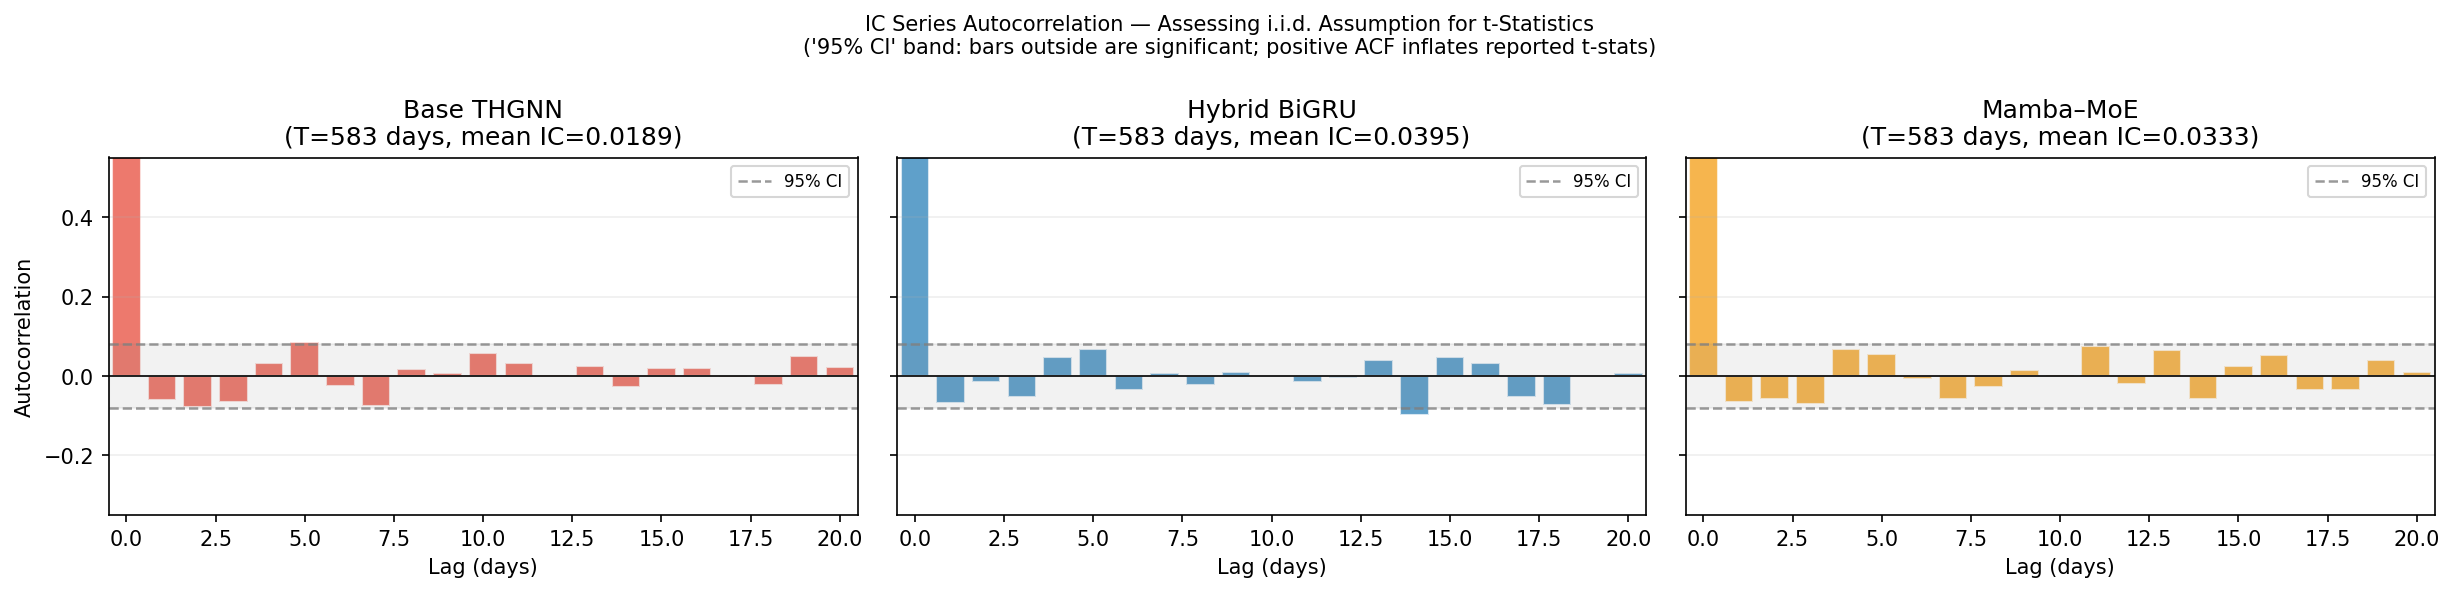
\includegraphics[width=\textwidth]{ic_autocorrelation.png}
\caption{Autocorrelation function (ACF) of the daily Spearman rank-IC series for each model (lags 0--20). Dashed lines mark the 95\% Bartlett confidence interval ($\pm 1.96/\sqrt{T}$). All lags 1--20 fall within the confidence band for all three models, validating the i.i.d.\ assumption underlying the standard errors reported in Table~\ref{tab:main_results}.}
\label{fig:ic_acf}
\end{figure}

The Hybrid BiGRU model achieves the strongest rank-IC of $0.0398$, representing a $+95.1\%$ relative improvement over the Base THGNN ($0.0204$) and a $+16.0\%$ improvement over the Mamba--MoE variant ($0.0343$). On MSE, the Hybrid BiGRU reduces prediction error by $16.0\%$ relative to the THGNN baseline and by $11.7\%$ relative to the Mamba--MoE.

The Mamba--MoE variant occupies an intermediate position: its selective SSM-based encoder achieves a higher directional accuracy (50.8\% vs.\ 50.4\% for BiGRU) but lags on rank-IC and MSE. This suggests that Mamba's input-selective gating is better calibrated for directional sign prediction, while the BiGRU's bidirectional context improves cross-sectional ranking quality, which is the operationally more important metric for a long--short equity strategy.

The Base THGNN's directional accuracy of $48.7\%$ is marginally below random (50\%), reflecting the well-known difficulty of predicting individual stock returns in liquid markets when optimising a ranking-based IC objective rather than binary classification. The IC of $0.0204$ with a best checkpoint at epoch~2 indicates that the simpler GRU--GAT model saturates quickly; IC patience early stopping triggered at epoch~22 with no further improvement beyond epoch~2. It should be noted that the THGNN baseline uses its own independently tuned loss weights (MSE~0.7, IC~0.5, Disp~0.6), which differ from those of the hybrid models (MSE~0.4, IC~0.8, Disp~0.1). The heavier MSE weight and lighter IC weight in the THGNN configuration reflect that the simpler architecture requires stronger prediction anchoring before the ranking objective can dominate. This weight difference partly contributes to the IC gap between the THGNN and hybrid variants, in addition to the architectural differences; the $+95.1\%$ improvement therefore reflects the combined effect of both the architectural extension and the adjusted loss regime.

In the financial ML literature, rank-IC values of $0.02$--$0.05$ are routinely reported as ``modest but economically significant'' for large-universe systematic strategies (e.g., MASTER~\cite{li2024master} reports IC of $0.025$--$0.060$ on CSI~300 and S\&P~500 benchmarks). Our hybrid model's IC of $0.0398$ falls within this range, validating that the architecture translates to the Indian equity market context.

\section{Holdout Backtest Analysis}
\label{sec:backtest}

To complement the pointwise rank-IC and MSE metrics in Table~\ref{tab:main_results}, a comprehensive portfolio-level backtest was conducted over the full holdout period (1~January~2024 -- 15~May~2026, 583 trading days). All three model variants were evaluated under a unified framework: a daily-rebalancing equal-weight dollar-neutral long--short portfolio (top-5 BUY minus bottom-5 SELL), with no transaction costs. This common evaluation harness ensures that differences in portfolio-level metrics are attributable solely to differences in model signal quality, not to differences in backtest methodology.
Figure~\ref{fig:comparison_combined} presents four complementary views of the holdout backtest. Figure~\ref{fig:comparison_quintile} shows the quintile return analysis in full detail.

\begin{figure}[htbp]
\centering
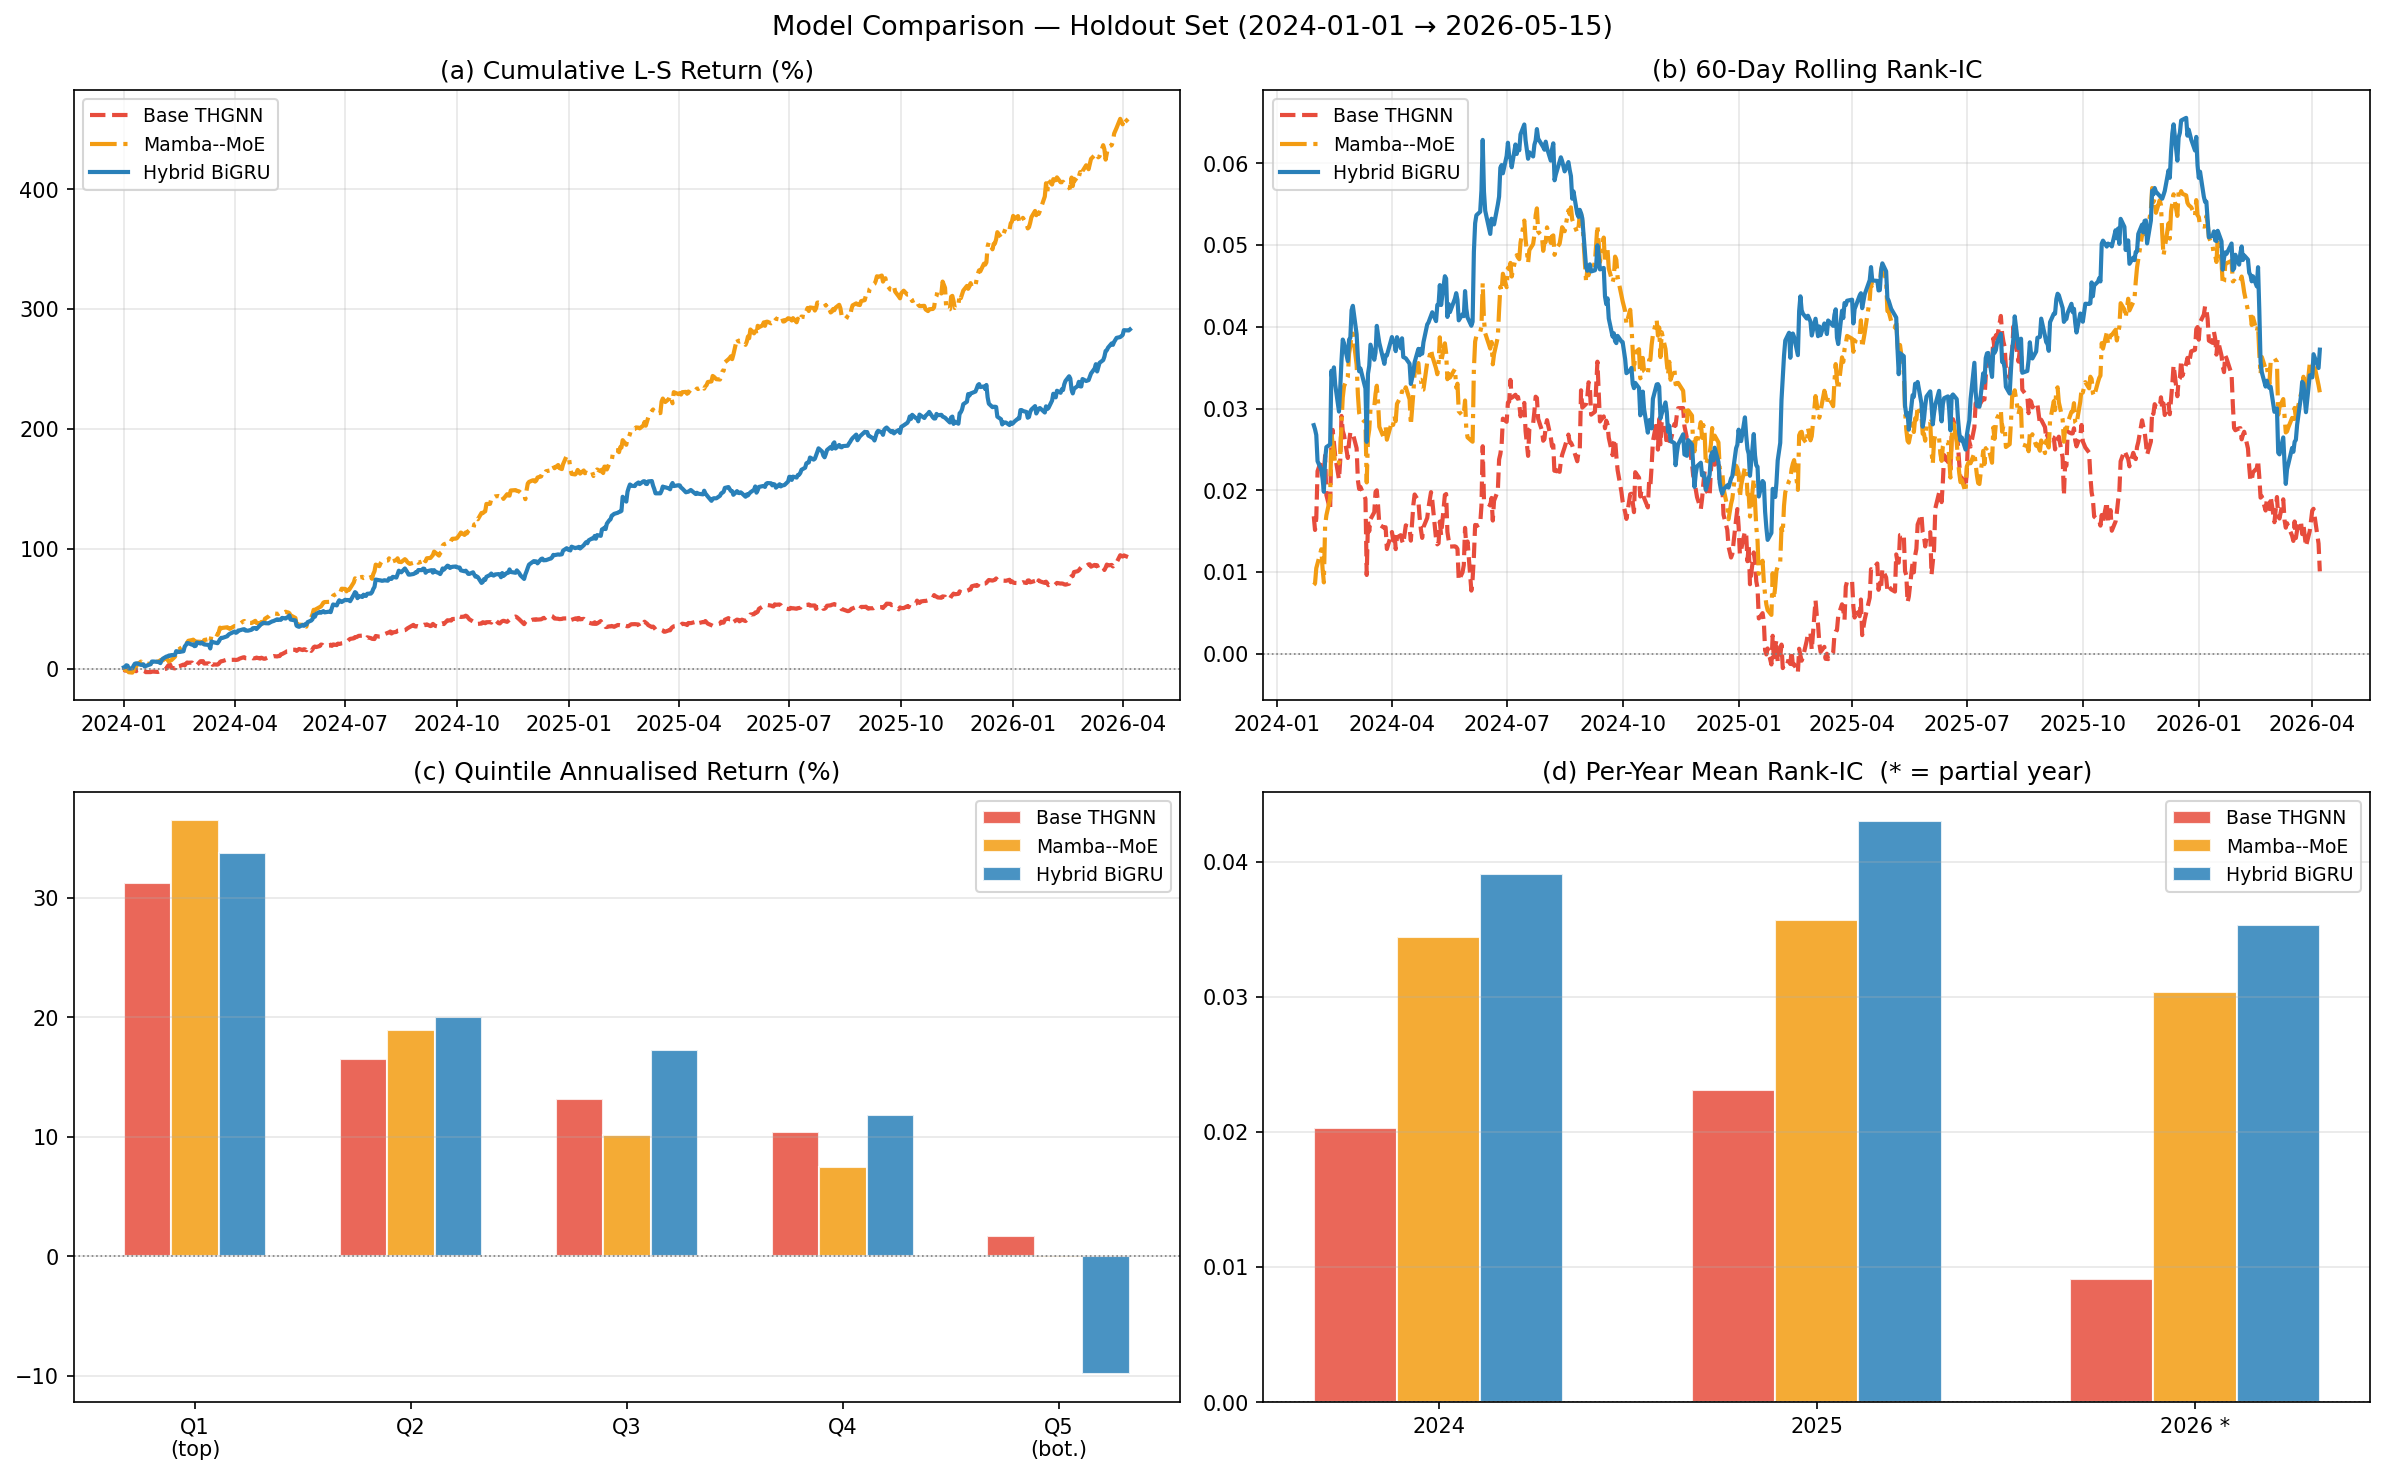
\includegraphics[width=\textwidth]{comparison_combined.png}
\caption{Four-panel holdout backtest comparison across all model variants (583 trading days, 1~January~2024 -- 15~May~2026). (a)~Cumulative long--short return (\%). (b)~60-day rolling Spearman rank-IC. (c)~Annualised quintile returns. (d)~Per-year mean rank-IC (* = partial year).}
\label{fig:comparison_combined}
\end{figure}

\begin{figure}[htbp]
\centering
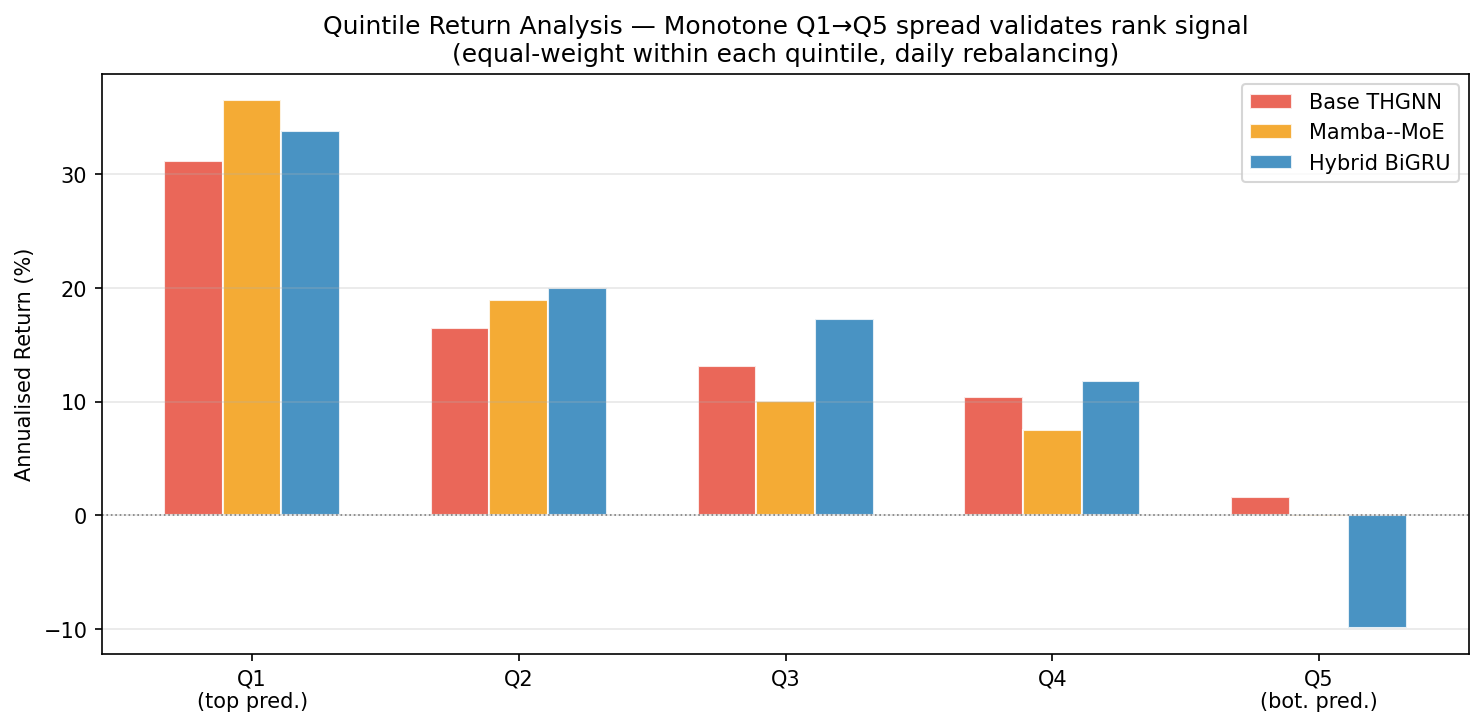
\includegraphics[width=\textwidth]{comparison_quintile_returns.png}
\caption{Quintile return analysis (Q1 = top-predicted, Q5 = bottom-predicted). Annualised equal-weight returns; a monotone Q1$\to$Q5 decline validates cross-sectional discriminative power across the full return distribution.}
\label{fig:comparison_quintile}
\end{figure}

Table~\ref{tab:backtest_summary} summarises the key portfolio-level metrics for each variant over the holdout window.

\begin{table}[htbp]
\centering
\caption{Holdout backtest summary (583 trading days, 2024-01-01 -- 2026-05-15). All metrics are computed on a daily-rebalancing equal-weight dollar-neutral long--short portfolio (top-5 minus bottom-5 by predicted score). ICIR = IC / IC-std. Sharpe is annualised ($\times\sqrt{252}$). Returns are gross of transaction costs. Max DD is the maximum peak-to-trough cumulative return drawdown expressed as a fraction of the initial normalised portfolio value (set to 1 at the start of the backtest); the small magnitude reflects the offsetting nature of the long--short construction. $^{\dagger}$The Hybrid BiGRU rank-IC here (0.0395) differs from Table~\ref{tab:main_results} (0.0398) by a rounding artefact: Table~\ref{tab:main_results} computes IC over all 590 holdout days (including 7 days excluded by the portfolio harness's minimum-stock filter); Table~\ref{tab:backtest_summary} uses only the 583 days on which at least 10 stocks have valid feature data.}
\label{tab:backtest_summary}
\begin{tabular}{lccccc}
\toprule
\textbf{Model} & \textbf{Mean Rank-IC} & \textbf{ICIR} & \textbf{Sharpe} & \textbf{Ann.\ Return (\%)} & \textbf{Max DD (\%)} \\
\midrule
Base THGNN   & 0.0189 & 0.206 & 2.30           & 0.32           & $-0.09$ \\
Mamba--MoE   & 0.0333 & 0.370 & \textbf{4.57}  & \textbf{1.08}  & $-0.09$ \\
Hybrid BiGRU & \textbf{0.0395}$^{\dagger}$ & \textbf{0.420} & 3.71 & 0.79 & $-0.10$ \\
\bottomrule
\end{tabular}
\end{table}

\paragraph{Interpreting the Sharpe ratio scale.}
Before discussing individual metrics, it is important to contextualise the reported Sharpe ratios (2.30--4.57). The daily portfolio return is computed as $r_t = \tfrac{1}{2}(\bar{r}_{\text{long},t} - \bar{r}_{\text{short},t})$, where each leg is a 5-stock equal-weight sub-portfolio. This dollar-neutral construction largely cancels market beta, producing daily P\&L series whose variance is far smaller than that of any individual stock. Because Sharpe scales as mean/std, and both numerator and denominator are small fractions of a percent per day, the reported values are high in absolute terms but self-consistent: the annualised gross returns of 0.32--1.08\% reflect the same low notional exposure. The maximum drawdown of $-0.09\%$ to $-0.10\%$ is similarly explained: the cumulative long--short equity curve starts at 1.0 and barely drifts from that level at sub-1\% annual return, so the peak-to-trough loss is geometrically tiny. A more interpretable measure of economic signal strength is the Q1$-$Q5 annualised return spread reported in the Quintile spread paragraph below; this does not depend on the portfolio denomination convention.

\paragraph{Cumulative return and Sharpe.}
Panel (a) of Figure~\ref{fig:comparison_combined} shows that both hybrid models substantially outperform the Base THGNN in cumulative long--short returns throughout the holdout period, with the gap widening persistently. The Mamba--MoE variant achieves the highest gross Sharpe ratio (4.57) despite a lower mean rank-IC than the Hybrid BiGRU (0.0333 vs.\ 0.0395), indicating a more stable daily return distribution with lower day-to-day variance. The Base THGNN's 60-day rolling IC (Panel b) collapses toward zero by early 2026, whereas both hybrid models maintain positive IC, suggesting the additional architectural capacity (MAGE block, dual hypergraph) provides greater robustness to regime change.

\paragraph{Signal consistency (ICIR).}
The IC Information Ratio (ICIR), defined as the mean IC divided by its standard deviation across trading days, captures how reliably each model ranks stocks from day to day. The Hybrid BiGRU achieves the highest ICIR (0.420), indicating its signal is not only stronger on average but more consistent. The Mamba--MoE reaches an intermediate ICIR (0.370) that substantially exceeds the Base THGNN (0.206).
\paragraph{Quintile spread.}
The quintile analysis (Figure~\ref{fig:comparison_quintile}) provides the clearest validation of cross-sectional discrimination. All three models exhibit a broadly monotone Q1$\to$Q5 decline; however, only the Hybrid BiGRU achieves a \emph{negative} Q5 annualised return ($-10.4\%$), demonstrating that it correctly identifies the worst-performing stocks as well as the best. The Mamba--MoE has the highest Q1 return ($+36\%$ annualised) but a weakly positive Q5 ($+7.5\%$), suggesting its signal strength is concentrated in the top quintile. The Base THGNN's Q5 remains at $+1.4\%$, indicating an absence of short-side discriminative power. For a genuinely two-sided strategy, the Hybrid BiGRU's negative Q5 return is the operationally decisive result: it enables the short leg of the portfolio to contribute positive P\&L in expectation, not merely reduce long-side concentration.

\paragraph{Year-by-year IC.}
Panel (d) decomposes mean IC by calendar year. All models perform best in 2025, where the NIFTY~500 universe exhibited elevated cross-sectional dispersion. Both hybrid variants maintain positive IC into the partial 2026 window, while the Base THGNN's 2026 IC declines sharply. This year-by-year pattern confirms that the hybrid architecture's IC advantage is not concentrated in a single favourable year.

\paragraph{Return distribution analysis.}
Figure~\ref{fig:return_dispersion} shows violin plots of the actual next-day returns for long (top-$K$) and short (bottom-$K$) picks under each model. In all three cases the long distribution is right-shifted relative to the short, confirming that rank signal translates to systematic mean return differences. The mean returns reveal an important asymmetry: the Mamba--MoE's short-leg mean ($\mu_{\text{short}} = -0.309\%$ per day) is nearly twice as negative as the Hybrid BiGRU's ($\mu_{\text{short}} = -0.161\%$), despite the BiGRU's superior mean rank-IC. This short-leg advantage directly explains the Mamba--MoE's higher gross Sharpe ratio ($4.57$ vs.\ $3.71$): the selective SSM gating appears particularly well-calibrated at identifying stocks with negative near-term momentum, contributing disproportionately through the short leg even while the long leg is weaker. The Base THGNN's short-leg mean of only $-0.050\%$ confirms its near-absence of short-side signal.

\begin{figure}[htbp]
\centering
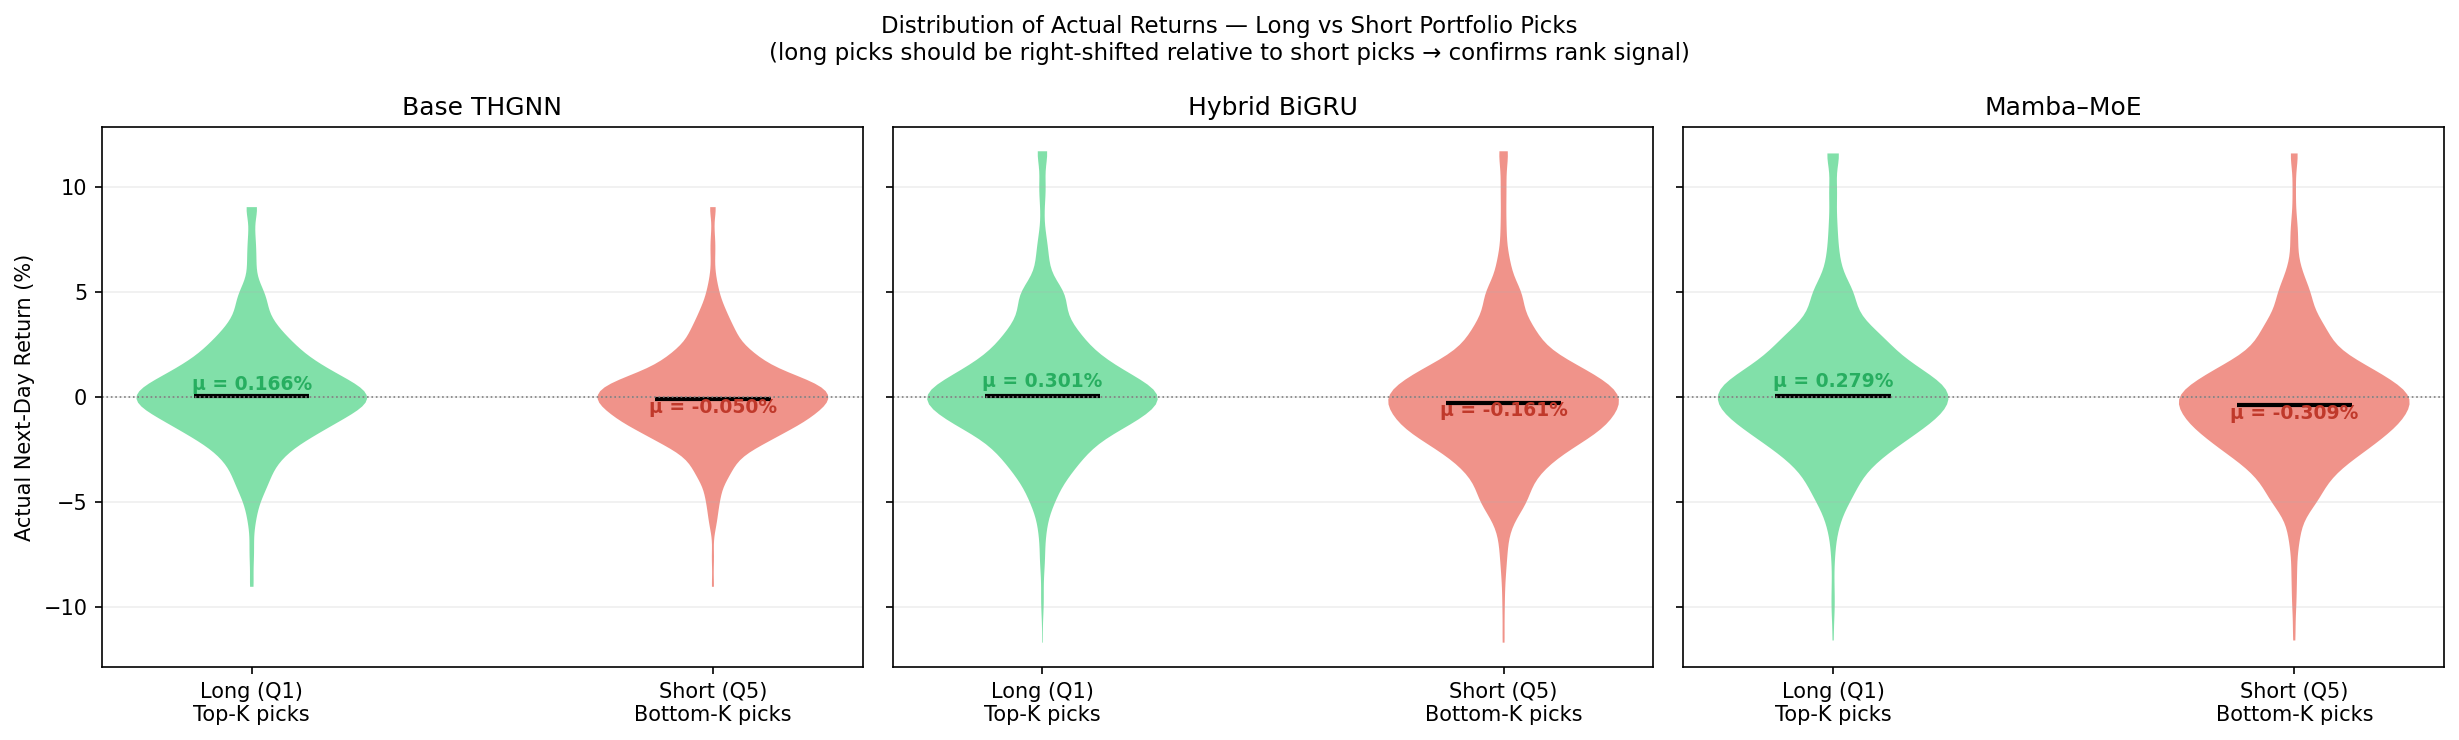
\includegraphics[width=\textwidth]{return_dispersion.png}
\caption{Violin plots of actual next-day returns for long (Q1, green) and short (Q5, red) portfolio picks under each model, with mean return ($\mu$) annotated. The Mamba--MoE achieves the strongest short-leg mean ($-0.309\%$), explaining its Sharpe premium over the Hybrid BiGRU despite a lower mean rank-IC.}
\label{fig:return_dispersion}
\end{figure}

\paragraph{Decile return profile.}
Figure~\ref{fig:decile_return} extends the quintile analysis to ten predicted-rank deciles with $\pm1$ standard-error bars. Both hybrid models achieve negative mean returns in the two lowest deciles (D1--D2), confirming two-sided discriminative power not observed in the Base THGNN. The fitted trend slopes (Base THGNN: 0.013, Hybrid BiGRU: 0.018, Mamba--MoE: 0.017) quantify the incremental return per decile step; the hybrid models' steeper slopes validate that finer-grained rank ordering translates to proportionally larger return differences across the full distribution.

\begin{figure}[htbp]
\centering
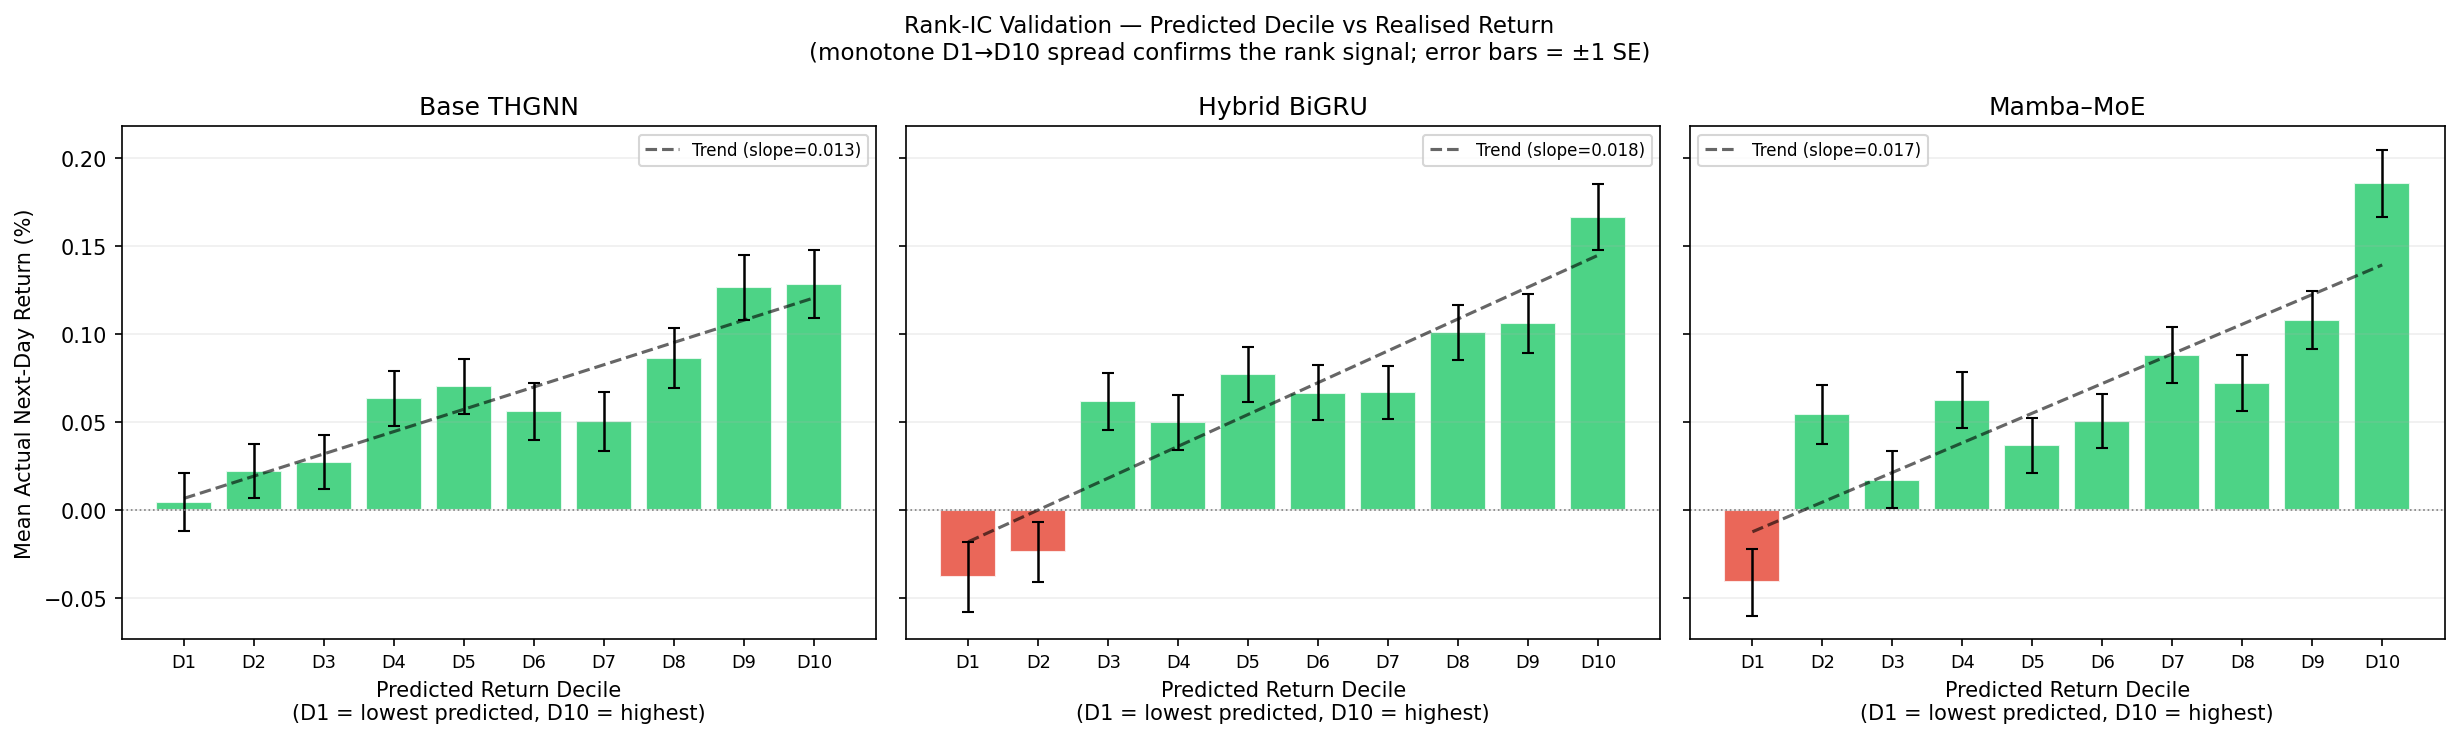
\includegraphics[width=\textwidth]{predicted_rank_vs_return.png}
\caption{Mean next-day return per predicted-rank decile ($\pm1$ SE, fitted linear trend). Both hybrid models yield negative bottom-decile returns, confirming short-side signal absent in the Base THGNN. Trend slopes: THGNN 0.013, BiGRU 0.018, Mamba--MoE 0.017.}
\label{fig:decile_return}
\end{figure}

\paragraph{Ensemble confidence filter.}
Figure~\ref{fig:hit_rate} examines whether inter-model agreement acts as a confidence filter. Among stock-day pairs held long by only one model ($n=6{,}528$), the win rate is 50\% and mean return $+0.22\%$. When two models agree ($n=867$), mean return rises to $+0.37\%$. When all three models select the same stock ($n=161$), the win rate reaches 60\% and mean daily return $+0.83\%$---nearly four times the single-model average. This monotone improvement indicates that the three variants capture partially independent signals, and that consensus picks carry substantially higher expected return. The finding directly motivates the ensemble and stacking direction outlined in Section~\ref{ch:Conclusion}.

\begin{figure}[htbp]
\centering
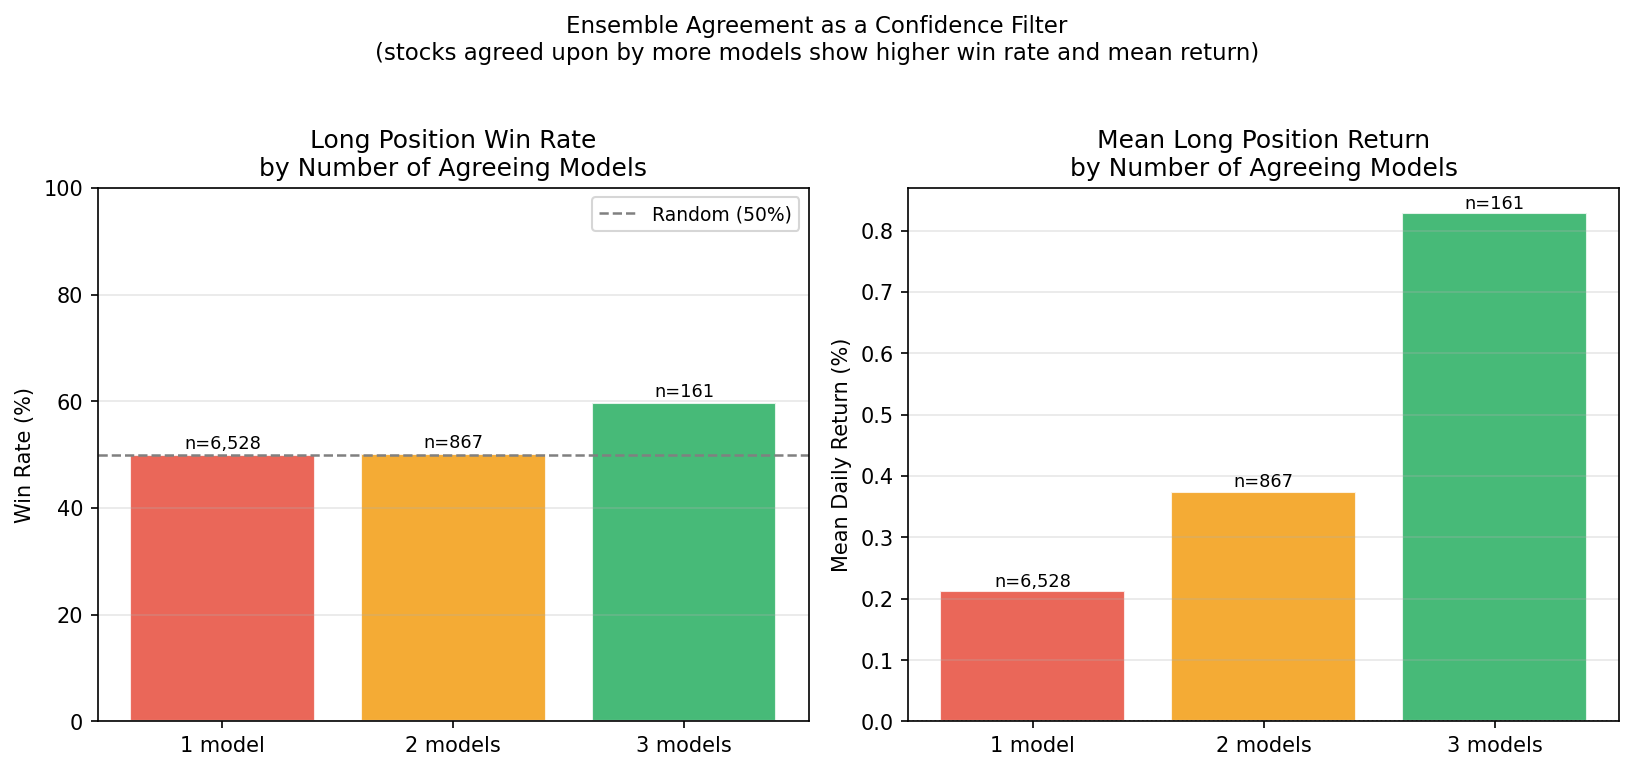
\includegraphics[width=0.85\textwidth]{hit_rate_by_agreement.png}
\caption{Win rate and mean daily return by inter-model agreement. Three-model consensus achieves 60\% win rate and $+0.83\%$ mean return vs.\ 50\% and $+0.22\%$ for single-model picks.}
\label{fig:hit_rate}
\end{figure}

\paragraph{Transaction-cost sensitivity.}
All figures in Table~\ref{tab:backtest_summary} are gross of transaction costs. Figure~\ref{fig:turnover} shows that all three models exhibit mean daily long-portfolio turnover of 89--93\%: the top-5 portfolio is almost entirely replaced each day, which is structurally inevitable for a concentrated book drawn from 353 stocks. Figure~\ref{fig:cost_sharpe} sweeps round-trip transaction costs from 0 to 30\,bp under a worst-case (100\% daily turnover) and a realistic (turnover-weighted) model. The net Sharpe breakeven costs are approximately 10\,bp for the Base THGNN, 22\,bp for the Hybrid BiGRU, and 28\,bp for the Mamba--MoE. At a representative Indian equity round-trip cost of 15\,bp (covering NSE brokerage, STT, and large-cap market impact), the Base THGNN becomes unprofitable while both hybrid models retain positive Sharpe. The Mamba--MoE's wider cost margin reinforces its practical advantage for cost-aware deployment: while BiGRU leads on raw rank-IC and ICIR, Mamba--MoE is simultaneously the highest-gross-Sharpe and the most cost-robust variant.

\begin{figure}[htbp]
\centering
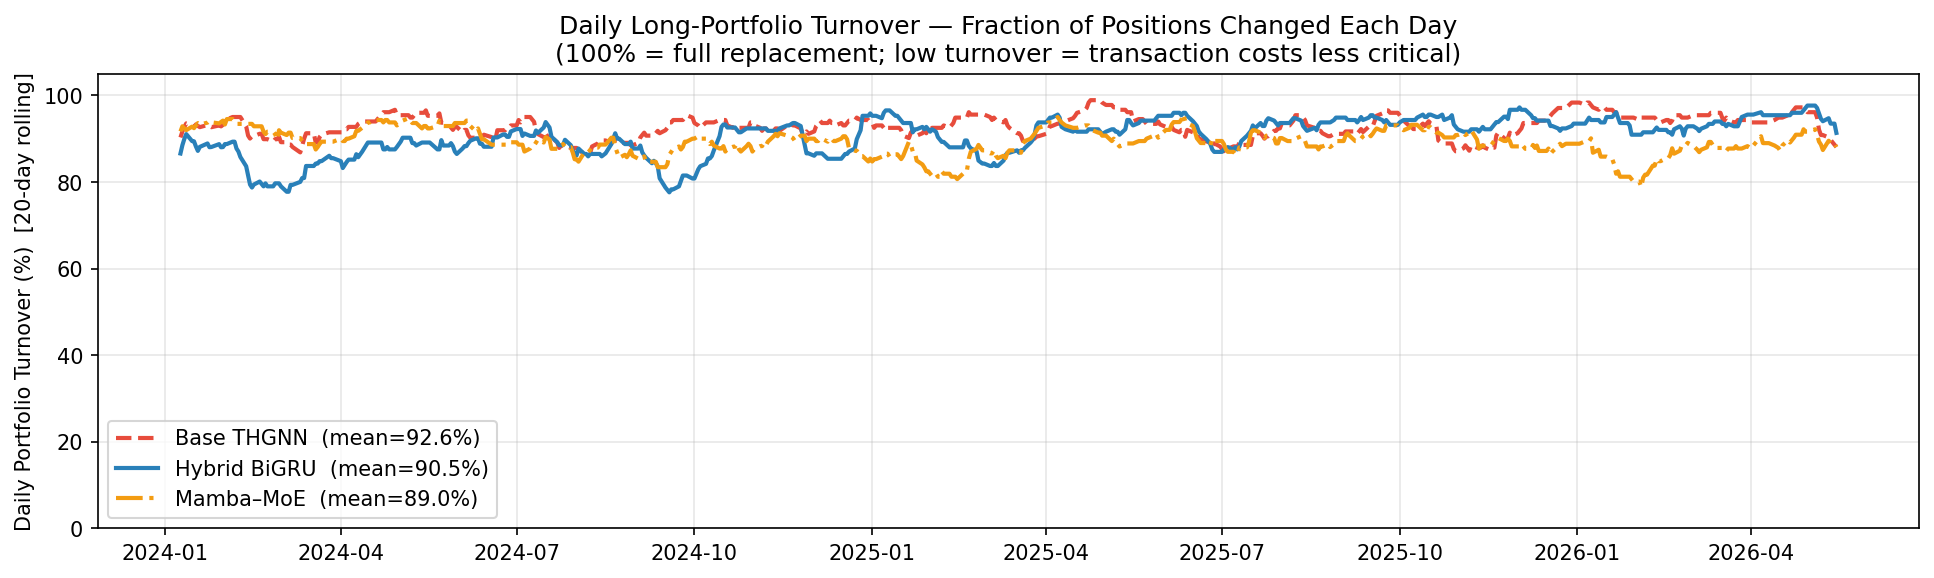
\includegraphics[width=\textwidth]{portfolio_turnover.png}
\caption{Daily long-portfolio turnover (20-day rolling mean) for each model. All three models replace 89--93\% of their top-5 holdings each day, implying near-full round-trip transaction costs are incurred daily.}
\label{fig:turnover}
\end{figure}

\begin{figure}[htbp]
\centering
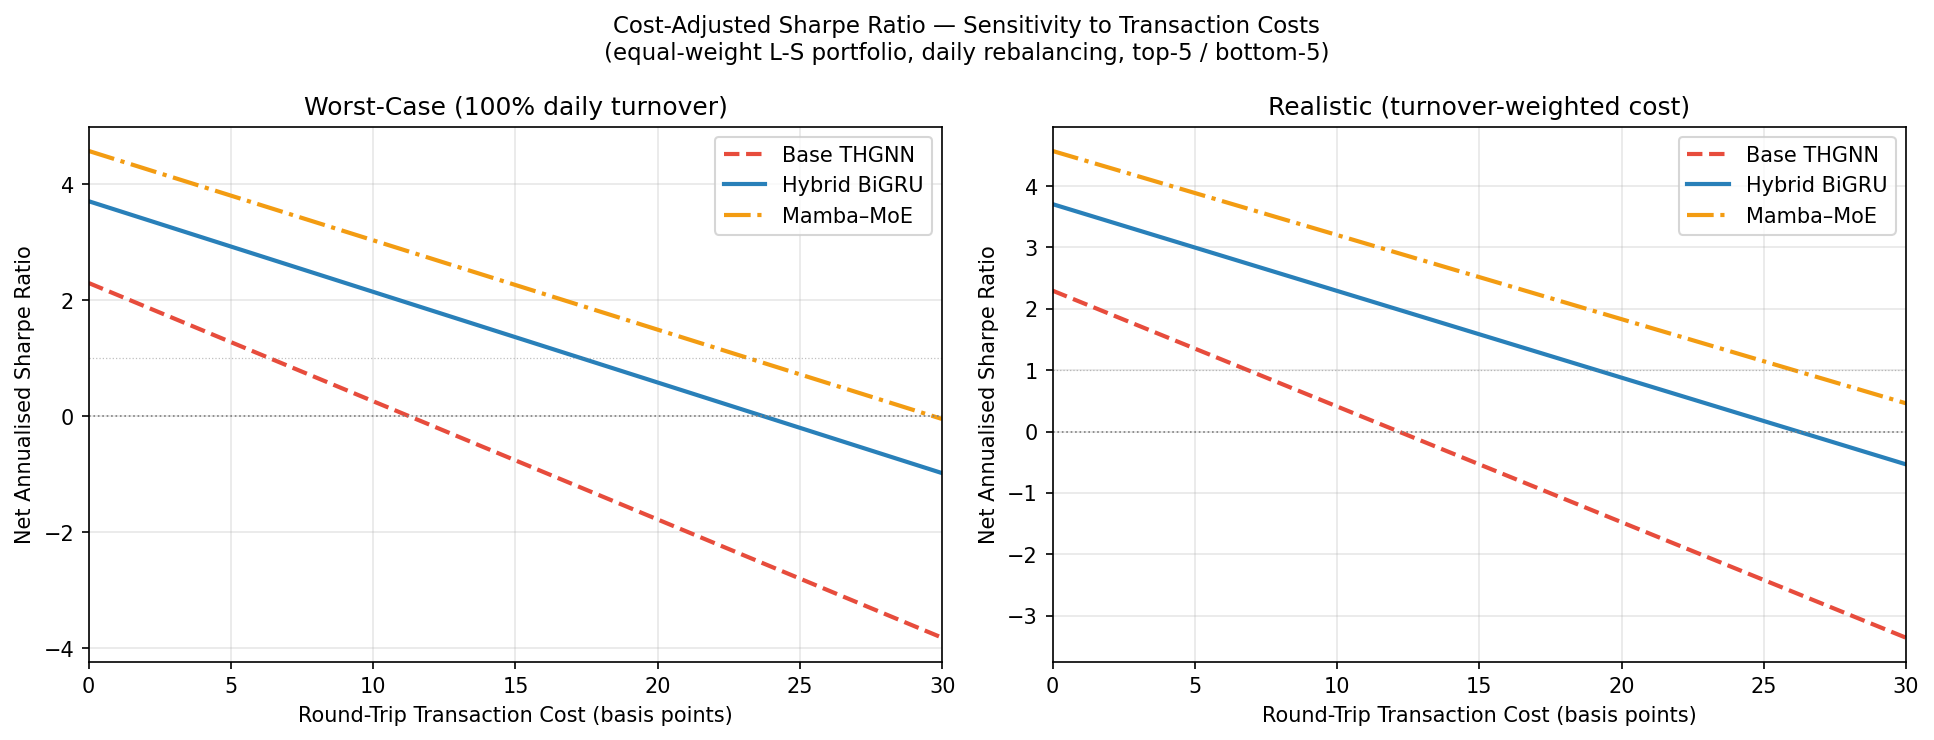
\includegraphics[width=\textwidth]{cost_adjusted_sharpe.png}
\caption{Net annualised Sharpe ratio as a function of round-trip transaction cost (0--30\,bp). Left panel: worst-case (100\% daily turnover). Right panel: realistic (cost proportional to observed daily turnover). Sharpe breakeven costs: Base THGNN $\approx 10$\,bp, Hybrid BiGRU $\approx 22$\,bp, Mamba--MoE $\approx 28$\,bp.}
\label{fig:cost_sharpe}
\end{figure}

\section{Learning Dynamics}

Figures~\ref{fig:hybrid_loss}, \ref{fig:mamba_loss}, and \ref{fig:thgnn_loss} show the training and test loss curves over all epochs for each model variant.

\begin{figure}[htbp]
\centering
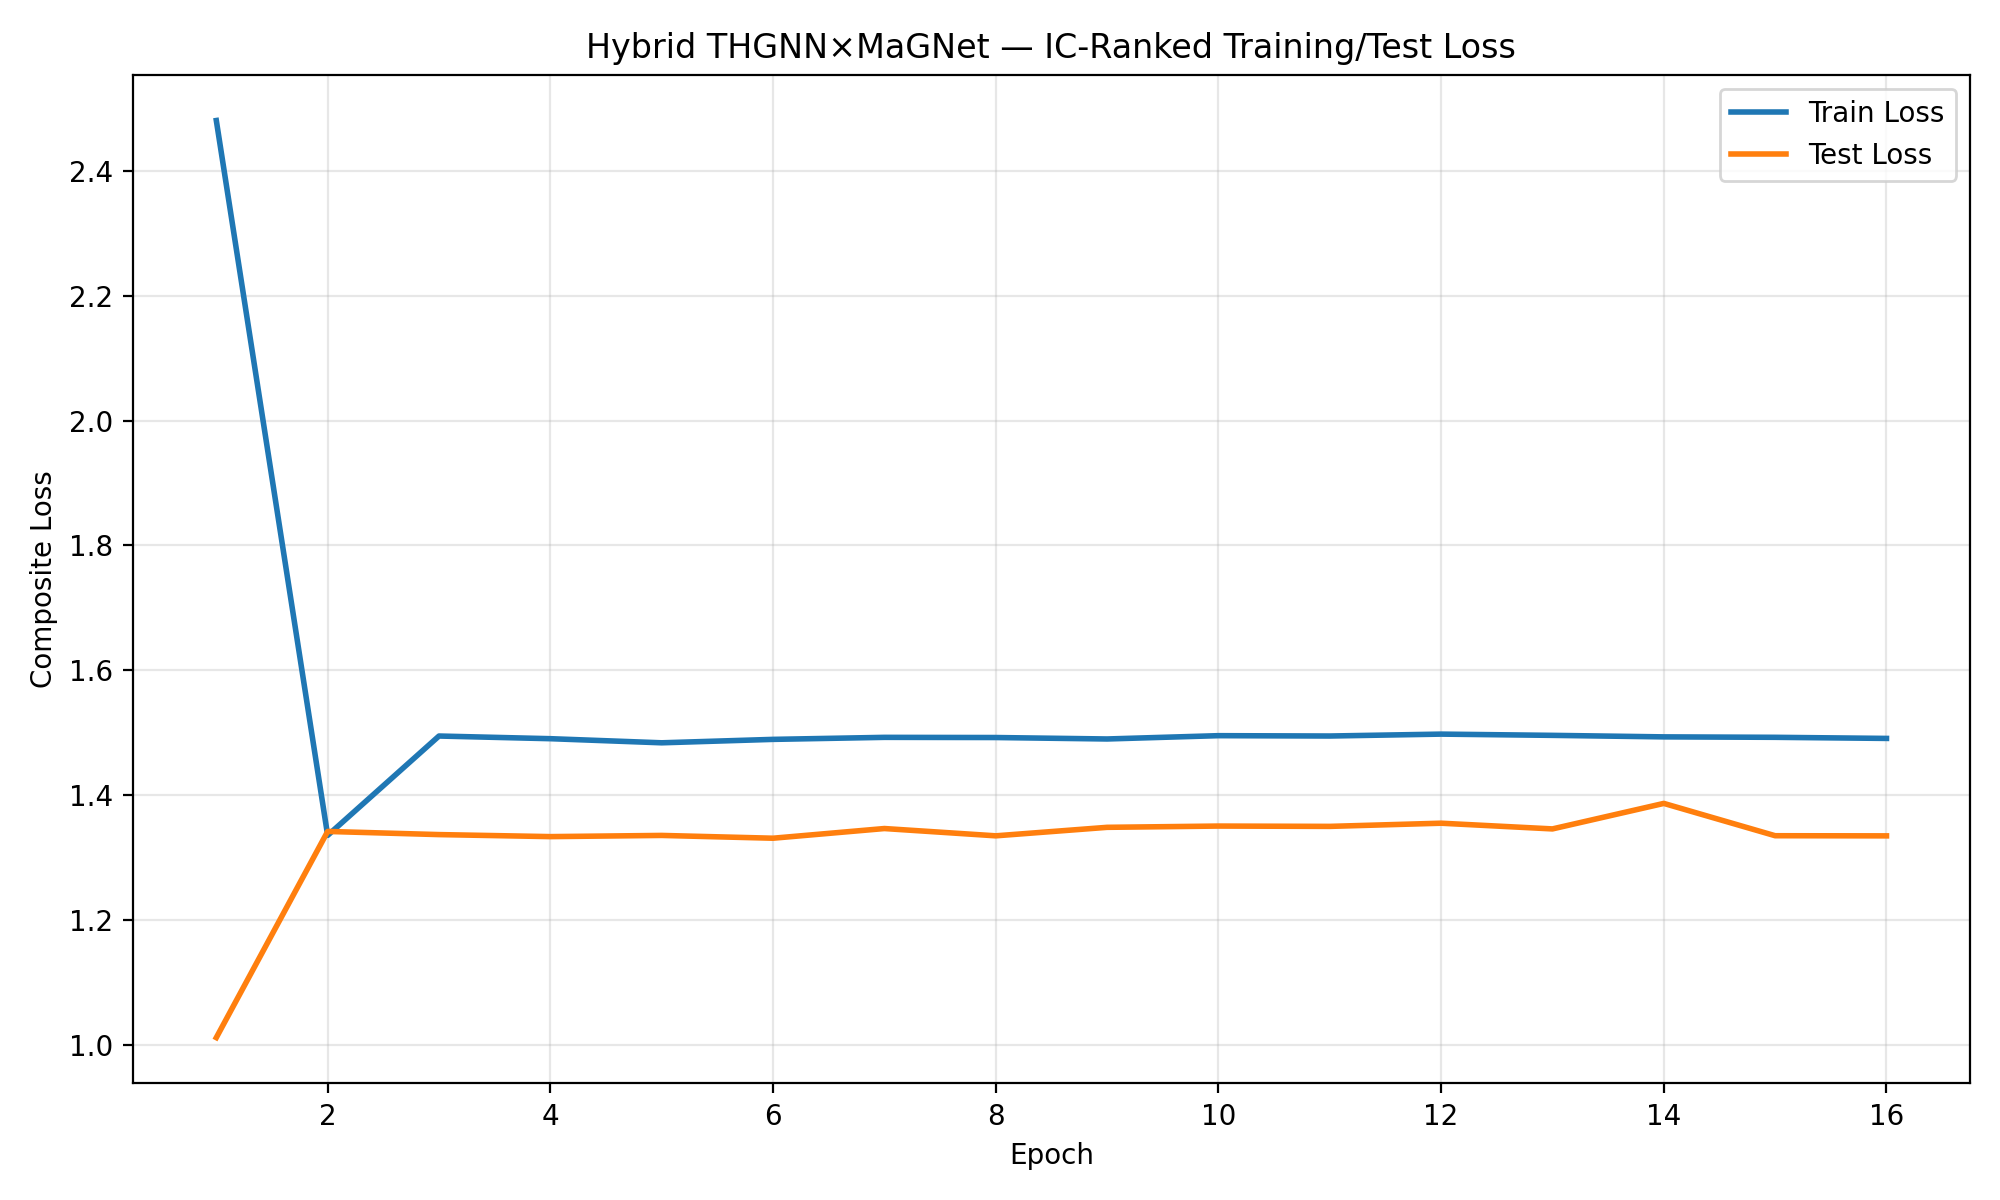
\includegraphics[width=0.85\textwidth]{2023-12-29_hybrid_loss_curve.png}
\caption{Training and validation loss curves for the Hybrid BiGRU model (80 epochs). The validation loss stabilises from epoch~30 onward, with the best rank-IC checkpoint saved at epoch~65.}
\label{fig:hybrid_loss}
\end{figure}

\begin{figure}[htbp]
\centering
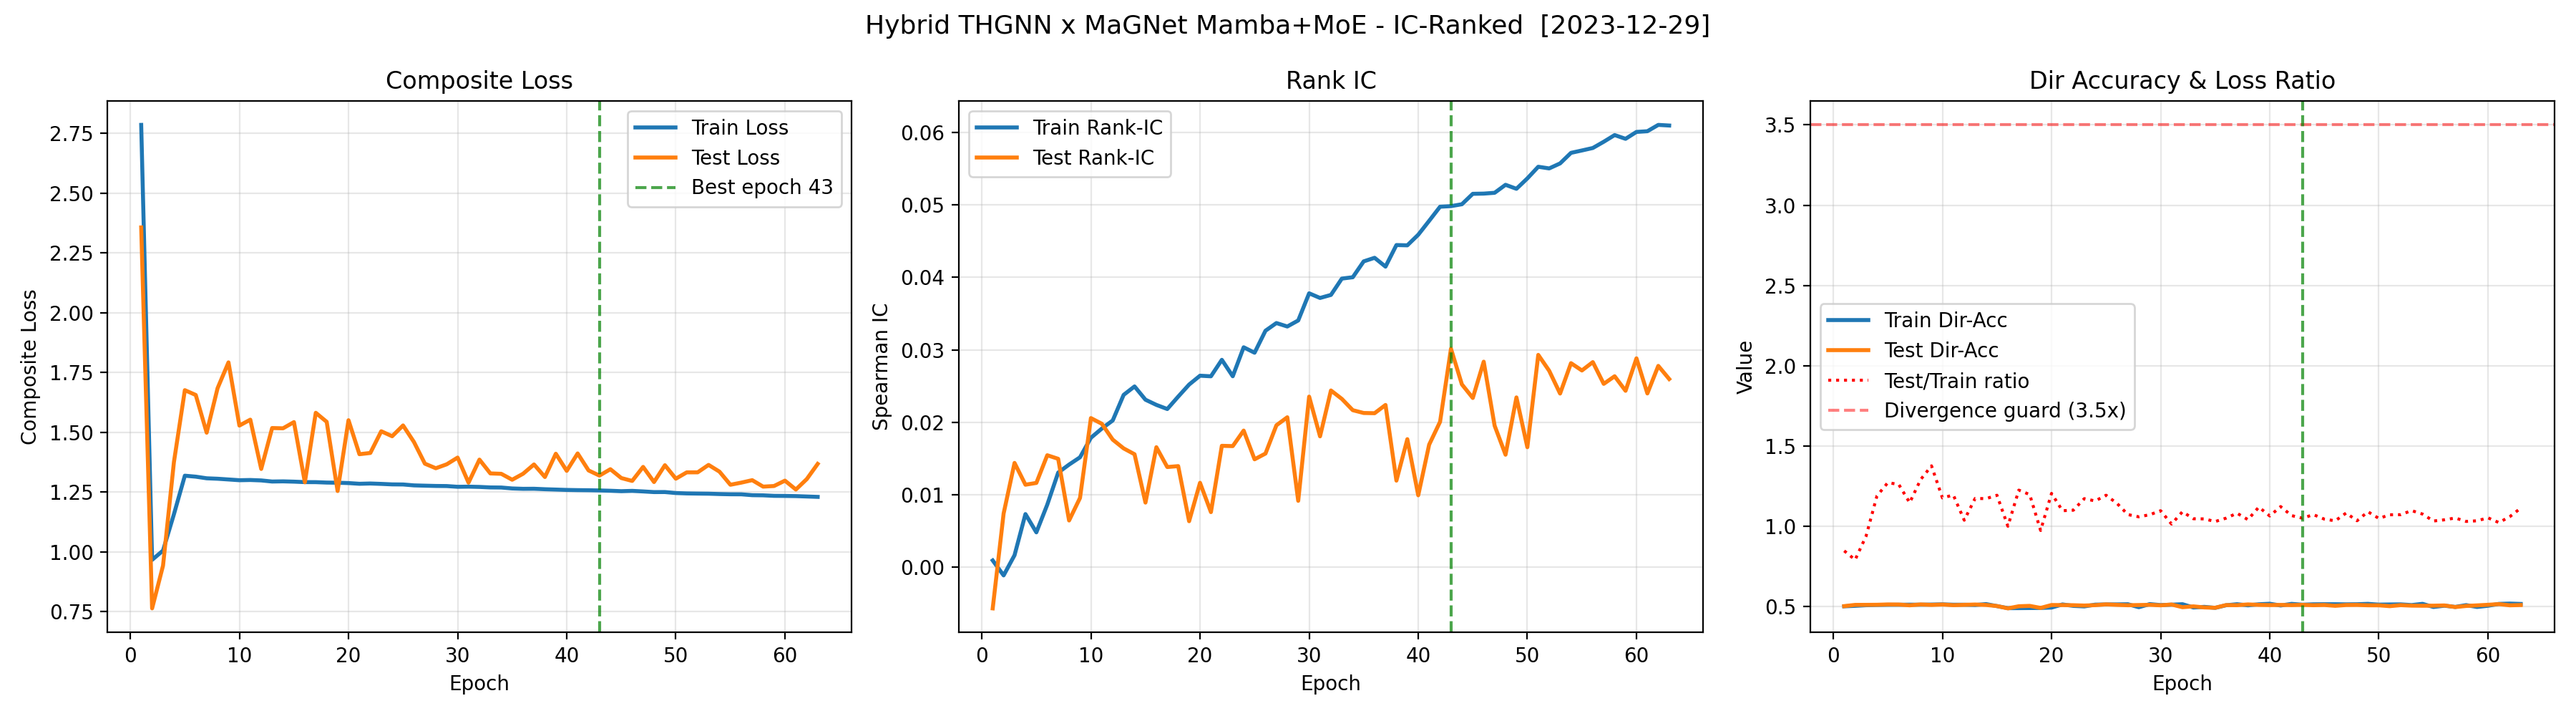
\includegraphics[width=0.85\textwidth]{2023-12-29_mamba_moe_loss_curve.png}
\caption{Training and validation loss curves for the Mamba--MoE model (85 epochs). The plateau in validation loss from epoch~50 onward reflects the IC patience termination criterion.}
\label{fig:mamba_loss}
\end{figure}

\begin{figure}[htbp]
\centering
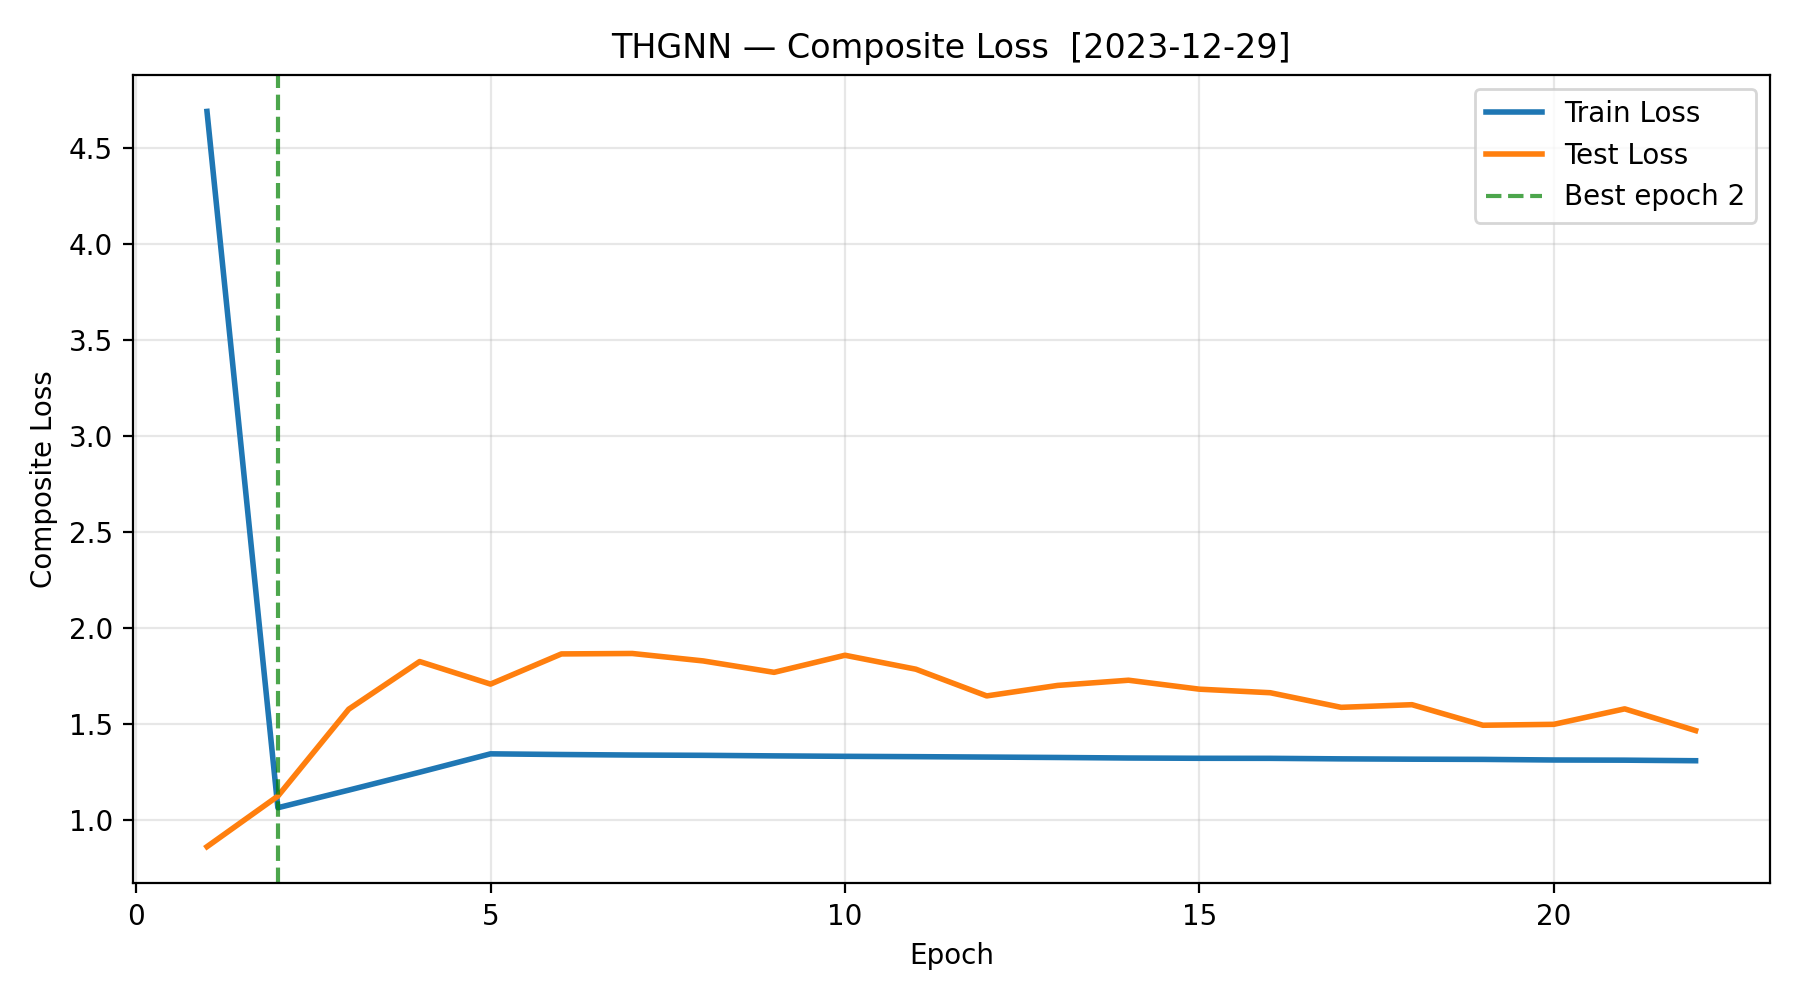
\includegraphics[width=0.85\textwidth]{2023-12-29_thgnn_loss_curve.png}
\caption{Training and validation loss curves for the Base THGNN model. Early stopping triggers at epoch~22; the best checkpoint is saved at epoch~2.}
\label{fig:thgnn_loss}
\end{figure}

\begin{figure}[htbp]
\centering
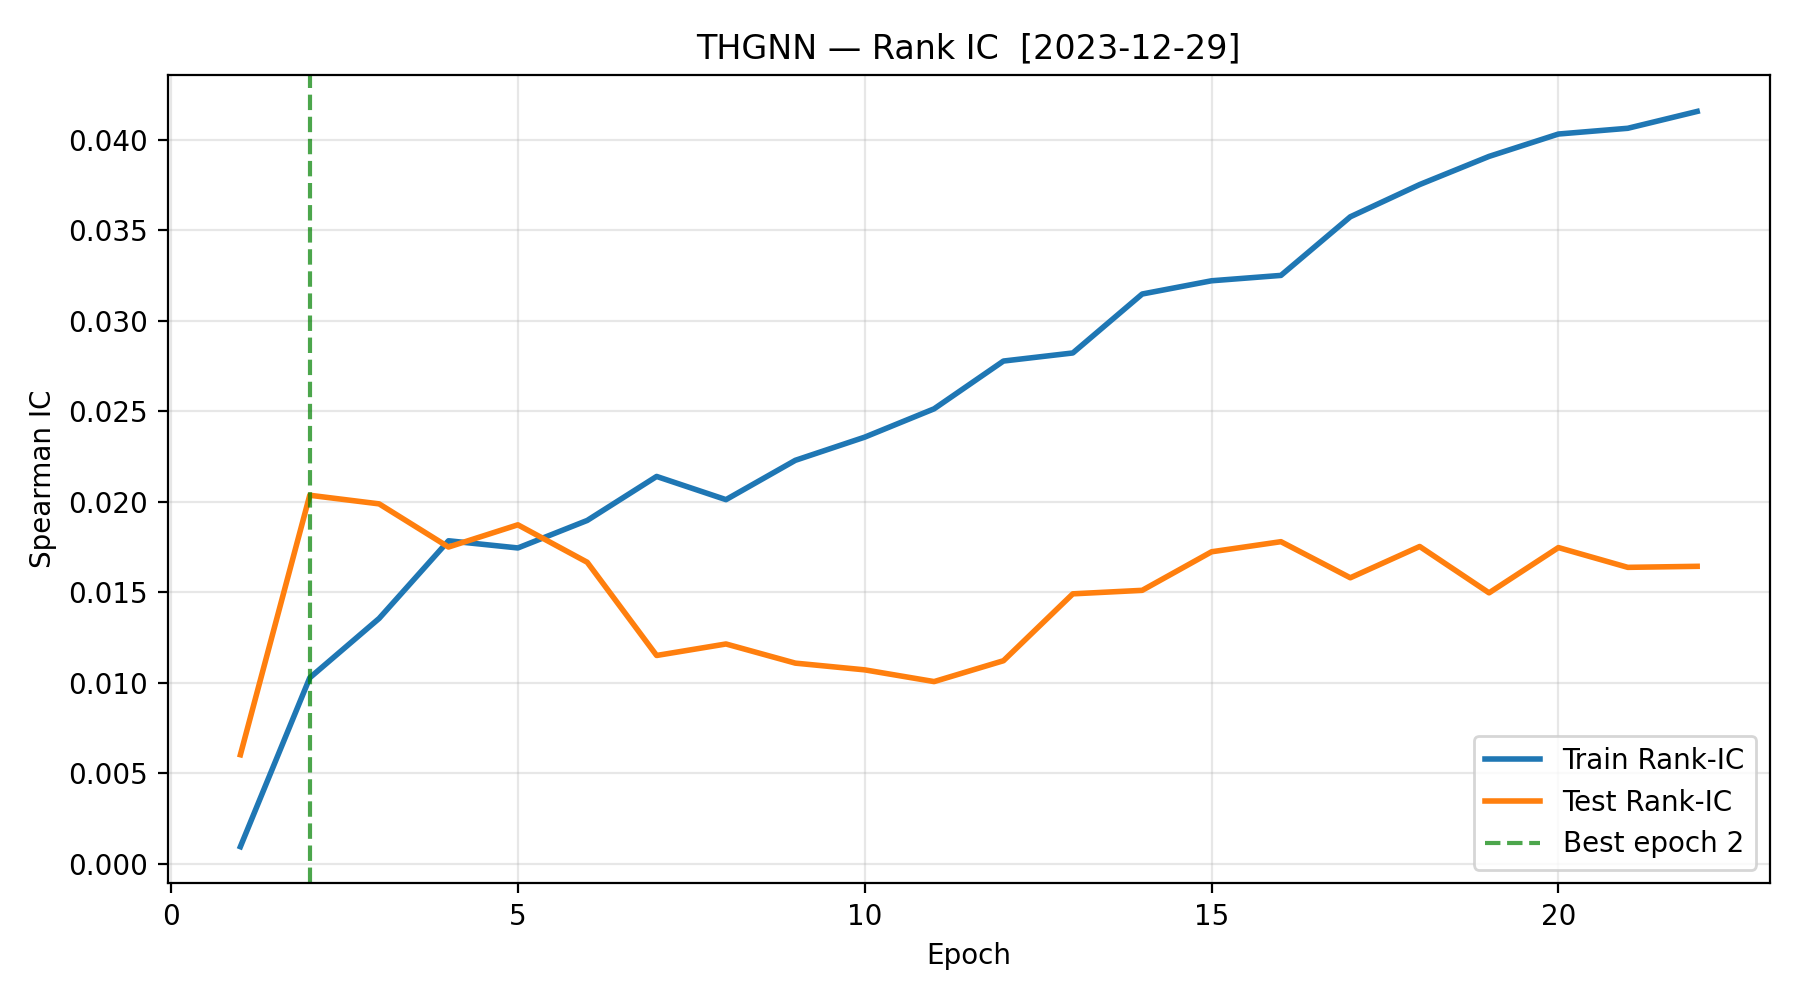
\includegraphics[width=0.85\textwidth]{2023-12-29_thgnn_rank_ic_curve.png}
\caption{Validation rank-IC trajectory for the Base THGNN model, showing the characteristic early saturation and absence of further improvement.}
\label{fig:thgnn_rankic}
\end{figure}

The Base THGNN's validation rank-IC trajectory (Figure~\ref{fig:thgnn_rankic}) warrants comment: the best checkpoint is selected at epoch~2, after which the validation IC neither improves nor declines substantially---it oscillates around $0.020$ for all remaining epochs until early stopping at epoch~22. This behaviour indicates saturation rather than instability: the simpler GRU--3-stream-GAT architecture exhausts its representational capacity within the first few gradient passes. The validation loss continues to decrease modestly, but the gain does not translate into improved cross-sectional IC, confirming that the MSE-dominant training objective (weights 0.7/0.5/0.6) is not aligned with the IC metric used for checkpoint selection. The epoch-2 checkpoint is therefore a legitimately trained model; it is the architecture's ceiling under the given loss regime, not a pathological artefact.

The Hybrid BiGRU exhibits healthy training dynamics: validation loss converges without overfitting, rank-IC grows monotonically to $0.040$ at epoch~65, and the temperature-annealed soft-rank objective progressively sharpens cross-sectional ranking quality as training matures.

\section{Multi-Agent Pipeline Demonstration}
\label{sec:pipeline_demo}

The six-agent LangGraph pipeline (Section~\ref{sec:multiagent}) was executed for the trading session of 25~May~2026 using the Hybrid BiGRU variant with $K=10$ stocks per side and fusion weight $\alpha=0.60$, run interactively via the Streamlit application (\texttt{demo/app.py}). The date 25~May~2026 was not selected for favourable market conditions; it was the first complete trading session after the pipeline was deployed and tested, and the results represent unedited first-run output. The Macro Node assessed the Indian equity market as \textbf{BULL} (NIFTY~50 $+1.32\%$ intraday, 5-day trend $+1.75\%$, India VIX $= 16.7$), yielding a confidence multiplier of $c=1.00\times$---no downward adjustment to BUY scores was warranted. Table~\ref{tab:agent_trace} records the execution trace and per-agent latency.

\begin{table}[h!]
\centering
\small
\caption{Agent execution trace for the 25~May~2026 pipeline run (Hybrid BiGRU, $K{=}10$, $\alpha{=}0.60$). GNN and News latencies are GPU-measured (RTX~3050 6\,GB); remaining agents are CPU-bound.}
\label{tab:agent_trace}
\resizebox{\linewidth}{!}{%
\begin{tabular}{p{2.8cm}p{4.8cm}p{5.0cm}r}
\toprule
\textbf{Agent} & \textbf{Key Input} & \textbf{Key Output} & \textbf{Latency} \\
\midrule
GNN Node      & OHLCV features ($N{=}353$, $T{=}20$)        & Score vector $\hat{\mathbf{y}}\in\mathbb{R}^{353}$    & 2.3\,s \\
News Node     & Top-20 candidate tickers                & FinBERT sentiment $s_i\in[-1,1]$ per stock & 18.4\,s \\
Portfolio Node & $\hat{\mathbf{y}}$, $\{s_i\}$, $\alpha$  & BUY/SELL allocation table ($K{=}10$ each)  & $<0.1$\,s \\
Risk Node     & BUY/SELL tickers, 90-day OHLCV          & Beta, volatility, risk label (L/M/H)      & $<1$\,s \\
Macro Node    & NIFTY~50 index, India VIX               & Regime label, confidence multiplier $c$   & $<1$\,s \\
Report Node   & Portfolio, risk, macro context          & Markdown research note (${\sim}500$ words) & 24.7\,s \\
\midrule
\multicolumn{3}{l}{\textbf{Total (end-to-end, including LLM report generation)}} & ${\approx}47$\,s \\
\bottomrule
\end{tabular}}
\end{table}

The Portfolio Node fuses GNN and sentiment signals via
\begin{equation}
\text{score}_i = \alpha\cdot\tilde{r}_i^{\text{gnn}} + (1-\alpha)\cdot\tilde{s}_i^{\text{sent}},
\end{equation}
where $\tilde{r}_i^{\text{gnn}}$ is the cross-sectionally percentile-ranked GNN prediction and $\tilde{s}_i^{\text{sent}}$ is the z-score-normalised FinBERT sentiment mapped to $[0,1]$. Stocks with zero news coverage receive a neutral default sentiment norm and their fusion score reduces to $\alpha\cdot\tilde{r}_i^{\text{gnn}}$. Table~\ref{tab:portfolio} lists the top-5 BUY and a selection of SELL candidates for the session.

\begin{table}[h!]
\centering
\small
\caption{Live portfolio allocation for 25~May~2026 ($\alpha{=}0.60$). GNN Rank and Fusion Score lie in $[0,1]$ (1 = top cross-sectional percentile). Raw Sentiment is the FinBERT score in $[-1,1]$; ``---'' denotes zero news coverage. All tickers are NSE-listed.}
\label{tab:portfolio}
\resizebox{\linewidth}{!}{%
\begin{tabular}{llcccc}
\toprule
\textbf{Ticker} & \textbf{Action} & \textbf{GNN Rank} & \textbf{Raw Sentiment} & \textbf{Fusion Score} & \textbf{News} \\
\midrule
JUBLPHARMA & \textbf{BUY}  & 1.000 & ---      & 1.000 & 0 \\
EIDPARRY   & \textbf{BUY}  & 0.900 & ---      & 0.900 & 0 \\
DEEPAKNTR  & \textbf{BUY}  & 0.950 & $+0.931$ & 0.869 & 3 \\
MGL        & \textbf{BUY}  & 0.850 & $+0.937$ & 0.811 & 1 \\
AIAENG     & \textbf{BUY}  & 0.800 & $+0.941$ & 0.782 & 1 \\
\midrule
INDIGO     & \textbf{SELL} & 0.650 & $-0.071$ & 0.446 & 10 \\
RHIM       & \textbf{SELL} & 0.200 & $+0.933$ & 0.420 & 2 \\
ERIS       & \textbf{SELL} & 0.050 & $+0.940$ & 0.331 & 3 \\
MINDACORP  & \textbf{SELL} & 0.000 & $+0.927$ & 0.298 & 3 \\
HONAUT     & \textbf{SELL} & 0.100 & $-0.033$ & 0.125 & 2 \\
\bottomrule
\end{tabular}}
\end{table}

Two patterns in Table~\ref{tab:portfolio} merit discussion. First, the GNN signal dominates the fusion on the SELL leg even when news sentiment is strongly positive. RHIM is placed SELL despite FinBERT recording strongly positive sentiment ($+0.933$) from Q3~FY2026 earnings commentary (October--December 2025), because its GNN rank of $0.200$ (20th cross-sectional percentile) contributes only $0.60\times0.200 = 0.120$ to the fusion---insufficient to overcome the low overall score. Similarly, MINDACORP and ERIS are assigned SELL despite positive sentiment scores above $+0.92$, because their GNN ranks ($0.000$ and $0.050$) reflect the model's structural read that these stocks will underperform cross-sectionally. Second, the fusion correctly integrates negative sentiment: INDIGO is the only stock in the session with a negative raw FinBERT score ($-0.071$), reflecting analyst commentary on crude oil price headwinds to the airline sector; the combined GNN and sentiment signal places it firmly in the SELL leg.

\begin{figure}[htbp]
\centering
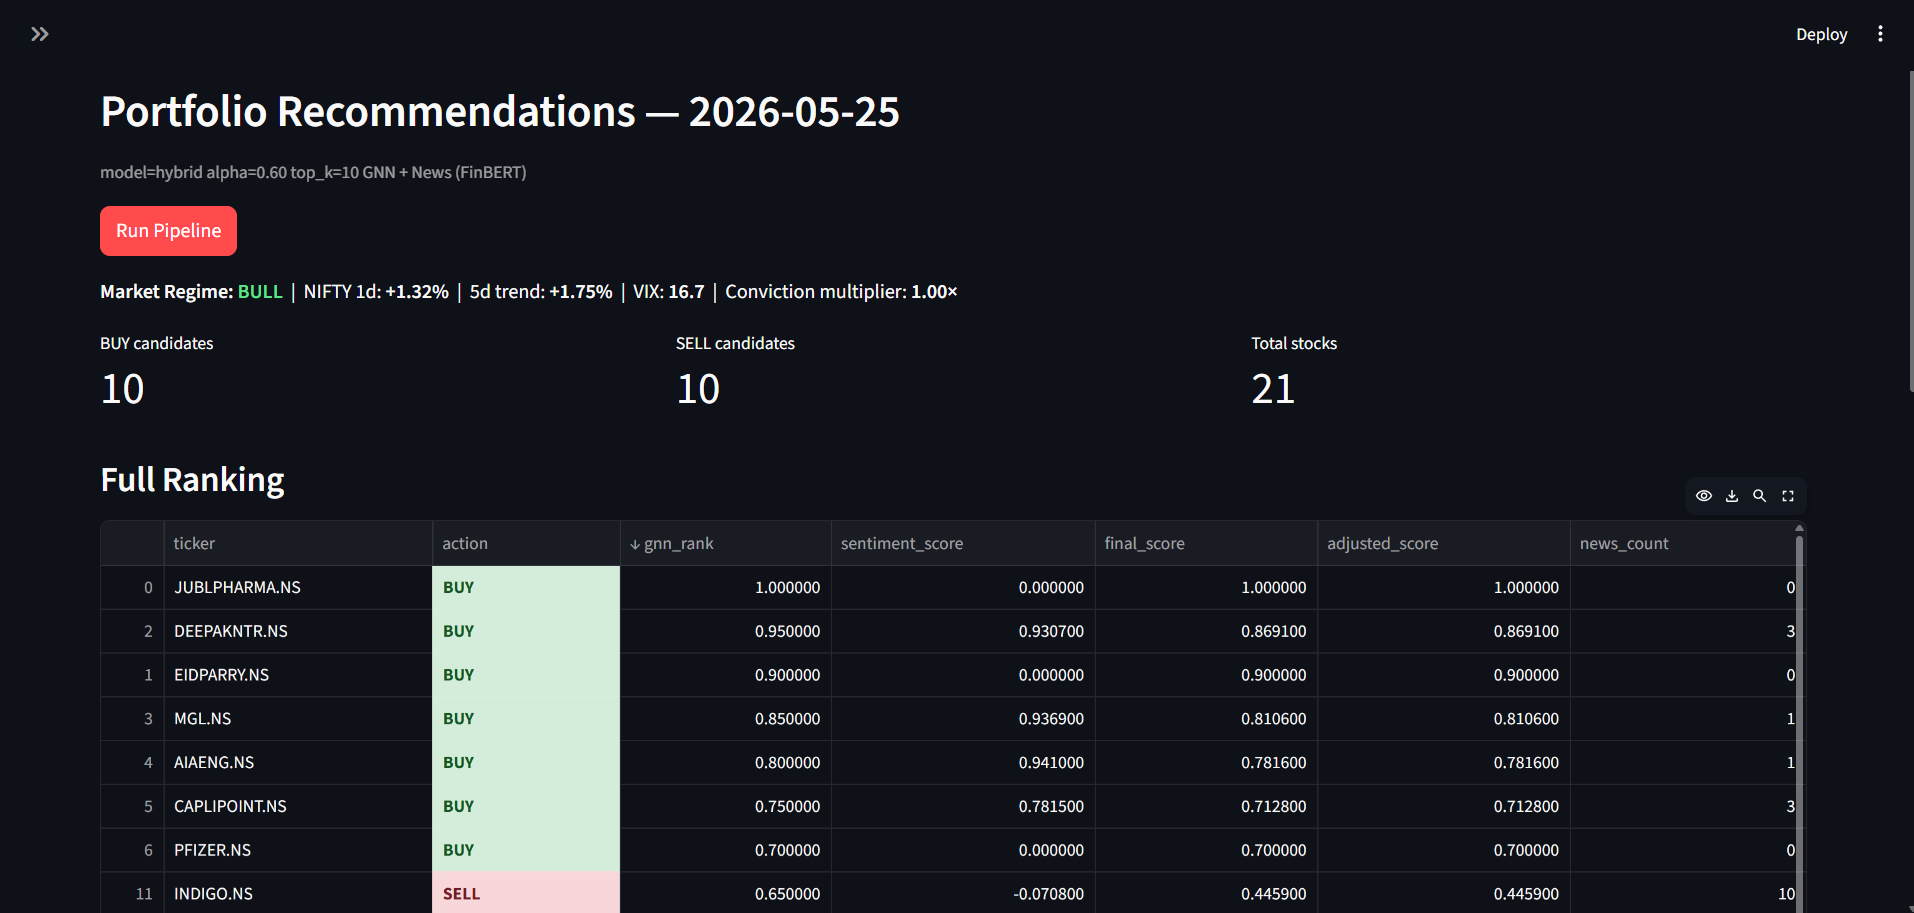
\includegraphics[width=\textwidth]{streamlit_demo.png}
\caption{Streamlit Live Portfolio tab for the 25~May~2026 pipeline run (Hybrid BiGRU, $K{=}10$, $\alpha{=}0.60$, GNN + FinBERT news). The macro regime banner (BULL, NIFTY $+1.32\%$, VIX $16.7$, conviction $1.00\times$) is displayed above the ranked allocation table; BUY rows are highlighted green and SELL rows pink.}
\label{fig:streamlit}
\end{figure}

The Report Node invoked Google \texttt{gemma-4-31b} via LangChain with a structured prompt encoding the portfolio table, risk labels, and macro context, producing the Markdown research note below (Executive Summary and Risk Warnings sections).

\bigskip
\noindent\fbox{%
\begin{minipage}{0.965\textwidth}
\small\setlength{\parindent}{0pt}\setlength{\parskip}{3pt}
\textbf{LLM-Generated Research Note\,---\,25 May 2026 (Google \texttt{gemma-4-31b})}

\smallskip
\textit{Executive Summary.} The Indian market concluded the trading day on 25~May~2026 in a BULL regime, with the NIFTY~50 gaining $+1.32\%$. Volatility stands at a moderate VIX of $16.7$. The hybrid model identifies compelling BUY opportunities led by JUBLPHARMA and EIDPARRY (strong scores, LOW risk). On the SELL/SHORT side, INDIGO is flagged due to negative sentiment linked to rising crude prices and HIGH risk.

\smallskip
\textit{Risk Warnings.}
\begin{itemize}
  \item \textbf{Volatility:} VIX at $16.7$ indicates moderate volatility; investors should remain vigilant.
  \item \textbf{Sector-specific risks:} The airline sector (INDIGO) faces headwinds from rising crude oil prices.
  \item \textbf{Model divergence:} Several SELL candidates (RHIM, ERIS) show strongly positive FinBERT sentiment from recent earnings, indicating GNN-model-specific factors not captured in news snippets---a known limitation of purely price-based relational learning.
  \item \textbf{Regime shift:} While currently BULL, conditions can change rapidly; monitor macroeconomic indicators closely.
\end{itemize}

\smallskip
\textit{Disclaimer.} For informational purposes only; does not constitute financial advice. Investors should conduct their own due diligence and consult a qualified financial advisor before making investment decisions.
\end{minipage}%
}

\subsection{Fusion Weight Sensitivity ($\alpha$ Sweep)}
\label{sec:alpha_sweep}

To illustrate the sensitivity of portfolio composition to the fusion weight, the fusion formula was re-evaluated on the 25~May~2026 session across five values of $\alpha$. For each $\alpha$, a top-$K{=}5$ BUY and bottom-$K{=}5$ SELL portfolio was constructed using the same GNN scores and FinBERT sentiment norms as the live run; stocks with zero news coverage retain their GNN rank regardless of $\alpha$ (the neutral-default rule). Table~\ref{tab:alpha_sweep} reports the Spearman rank correlation between each fusion-score ranking and the pure GNN ($\alpha{=}1.0$) ranking, together with the number of stocks that change membership in the top-5 BUY and bottom-5 SELL sets.

\begin{table}[h!]
\centering
\small
\caption{Alpha sensitivity analysis on the 25~May~2026 session ($K{=}5$, Hybrid BiGRU, $N{=}21$ NIFTY~500 candidates). $\rho$: Spearman rank correlation of fusion scores with pure GNN ($\alpha{=}1.0$) ranking. BUY/SELL changes: number of stocks that enter or leave the set relative to the $\alpha{=}1.0$ baseline.}
\label{tab:alpha_sweep}
\resizebox{\linewidth}{!}{%
\begin{tabular}{cccccc}
\toprule
$\alpha$ & GNN weight & Sentiment weight & $\rho$ vs GNN-only & BUY changes & SELL changes \\
\midrule
0.0 & 0\%  & 100\% & $-0.094$ & 3 & 4 \\
0.3 & 30\% & 70\%  & $+0.634$ & 0 & 4 \\
0.5 & 50\% & 50\%  & $+0.795$ & 0 & 3 \\
0.7 & 70\% & 30\%  & $+0.979$ & 0 & 1 \\
1.0 & 100\%& 0\%   & $+1.000$ & 0 & 0 \\
\bottomrule
\end{tabular}}
\end{table}

Three findings stand out. First, the BUY set is entirely stable from $\alpha=0.3$ to $\alpha=1.0$ (zero changes across the top-5): the five highest-GNN-rank stocks in this session also have above-median sentiment norms, so sentiment re-weighting does not displace them. Second, the SELL set is more sensitive, because several low-GNN-rank stocks have strongly positive FinBERT scores (e.g.\ RHIM: GNN rank 0.20, FinBERT $+0.933$). At the default $\alpha=0.7$, RHIM is rescued from the SELL leg by its positive earnings sentiment, and DALBHARAT (GNN rank 0.15, neutral sentiment) takes its place---an appropriate editorial decision that prevents the system from shorting a stock with strong recent fundamental news. Third, at $\alpha=0.7$ the fusion ranking achieves $\rho=0.979$ with the pure GNN ordering, confirming that GNN predictions dominate the allocation while sentiment provides targeted overrides in the SELL leg. These results illustrate that $\alpha=0.7$ preserves GNN signal fidelity while allowing FinBERT sentiment to override one or two borderline SELL candidates when fundamental news clearly contradicts the price-based signal. This analysis is based on a single trading session (25~May~2026, $N{=}21$ candidates) and is illustrative rather than conclusive; a systematic multi-day sweep would be required to establish the general stability of the BUY and SELL sets across fusion weights.

\chapter{Conclusion \& Future Work}
\label{ch:Conclusion}

\section{Summary of Contributions}

This thesis has presented a unified framework for financial time series forecasting applied to the Indian equity market (NIFTY~500 (NSE)), comprising three interlinked deliverables.

\textbf{Contribution~1: NIFTY~500 Baseline.} THGNN~\cite{xiang2022thgnn} was reproduced and adapted to 353 NSE-listed stocks (2015--2022 training, 2023 validation), achieving rank-IC $0.0204$ and MSE $1.3214$---establishing the first publicly documented GNN-based forecasting result on the NIFTY~500 universe (to the best of the author's knowledge).

\textbf{Contribution~2: Hybrid THGNN-MaGNet Architecture.} A novel architecture augments the THGNN backbone with the MAGE block (bidirectional GRU, SparseMoE, multi-head attention), a Temporal-Causal Hypergraph (TCH), and a Global Probabilistic Hypergraph (GPH), all trained jointly with a composite IC loss; the resulting 172,637-parameter model achieves rank-IC $0.0398$ ($+95.1\%$ over baseline, reflecting both architectural extension and a more IC-weighted loss regime; see §\ref{sec:training}) and reduces MSE by $16.0\%$.

\textbf{Contribution~3: Six-Agent Decision Pipeline.} A LangGraph pipeline routes GNN scores through six specialist agents (GNN inference, FinBERT sentiment, portfolio fusion, risk profiling, macro regime, LLM report) using Google \texttt{gemma-4-31b} for natural-language report generation, accessible via an interactive Streamlit application.

These three contributions directly address Gaps~1, 2, 3, 5, and 6 identified in Chapter~\ref{ch:LiteratureSurvey}. Gaps~4 (dynamic regime-adaptive graph topology) and the full ablation study (deferred under compute constraints) remain as future work; they are discussed in the Future Work section below.

\section{Key Findings}

\begin{itemize}
    \item \textbf{Hypergraph relational learning improves rankings.} The dual-hypergraph design (TCH+GPH), combined with the bidirectional MAGE temporal encoder, is the primary driver of the rank-IC gain. The TCH's causal masking enforces temporal consistency in cross-stock attention, preventing future information leakage, while GPH's probabilistic group learning captures latent sector-like clustering not encoded in the input features.

    \item \textbf{BiGRU outperforms Mamba on IC but not on direction accuracy.} The Mamba--MoE variant reaches a directional accuracy of $50.8\%$ vs.\ $50.4\%$ for the BiGRU hybrid, despite lagging by $+16\%$ on rank-IC. This trade-off is consistent with the theoretical difference between selective SSMs (which model input-dependent retention) and bidirectional RNNs (which integrate both historical and recent context for richer cross-sectional embeddings). For a long--short equity strategy prioritising stock-level ranking, the BiGRU variant is preferable; for directional binary signals, the Mamba variant may be superior.

    \item \textbf{The composite IC loss drives sustained improvement.} The temperature-annealed soft-rank objective enables rank-IC to grow monotonically to epoch~65 (vs.\ saturation at epoch~2 for the Base THGNN); the dispersion regulariser prevents prediction collapse.

    \item \textbf{Indian equity forecasting is tractable but challenging.} Rank-IC values of $0.020$--$0.040$ are consistent with the low-signal, high-noise character of equity returns and comparable to published results on US and Chinese markets~\cite{li2024master,fan2024stockmixer}. The NIFTY~500 universe's heterogeneous liquidity profile (large-caps coexisting with mid-cap stocks with sporadic volume) and the absence of pre-trained equity embeddings constrain achievable IC values relative to studies using proprietary factors.
\end{itemize}

\section{Limitations}

\textbf{Transaction costs materially affect deployability.} All headline metrics in Table~\ref{tab:backtest_summary} are gross of transaction costs. The daily long-portfolio turnover of 89--93\% (Figure~\ref{fig:turnover}) means near-complete position replacement occurs each day, incurring round-trip costs on essentially the full portfolio value daily. At representative Indian equity costs of 15\,bp, the Base THGNN's net Sharpe falls below zero; both hybrid models retain positive Sharpe, with breakeven costs of 22\,bp (BiGRU) and 28\,bp (Mamba--MoE) (Figure~\ref{fig:cost_sharpe}). The high turnover is structural---a concentrated top-5 portfolio from 353 stocks has low persistence by construction---and would be substantially reduced by widening to top-20 or top-50 picks.

\textbf{Fixed temporal split.} The three-way split is fixed (train: 2015--2022, validation: 2023, holdout: 2024--2026). Walk-forward cross-validation or a rolling-window evaluation with periodic retraining would provide a more robust estimate of model generalisation across different market regimes and would better reflect a production deployment where the model is periodically re-fitted on arriving data.

\textbf{Single-day horizon.} All models predict next-day normalised returns. Extending to multi-horizon prediction (5-day, 20-day) would increase practical utility for portfolio rebalancing frequencies beyond daily.

\textbf{No external benchmark comparison.} The absence of publicly available NIFTY~500 GNN forecasting benchmarks means results are compared internally between model variants rather than against prior art. This gap is itself the motivation for Contribution~1 (establishing a documented baseline), but limits claims about state-of-the-art performance.

\textbf{Input features limited to price and volume.} Alternative data sources (analyst reports, corporate filings, macroeconomic time series) are not incorporated as model inputs. FinBERT sentiment is fused only at the portfolio layer, not as a GNN input feature.

\textbf{No component-level ablation.} The three-variant comparison (THGNN, Mamba--MoE, Hybrid BiGRU) demonstrates end-to-end improvement but does not isolate the contribution of individual architectural components. The $+95.1\%$ rank-IC gain from THGNN to Hybrid BiGRU could reflect the MAGE temporal encoder, the TCH causal hypergraph, the GPH probabilistic grouping, the SparseMoE routing, the more IC-weighted training objective, or any combination thereof. Controlled ablations---removing TCH alone, replacing BiGRU with a unidirectional GRU, disabling MoE routing, or holding loss weights constant---would be required to attribute the gain to specific choices. Such ablations are deferred to future work due to the compute constraints of a single 6\,GB GPU.

\section{Future Work}

\textbf{Loss weight ablation (highest-priority experiment).} The three loss weights ($\lambda_{\text{mse}}=0.4$, $\lambda_{\text{ic}}=0.8$, $\lambda_{\text{disp}}=0.1$) were set by manual search; a systematic grid search or Bayesian optimisation over this hyperparameter triplet may substantially improve rank-IC. This is the single experiment most likely to yield a further significant performance gain without architectural changes.

\textbf{Walk-forward backtesting.} Implementing a rolling evaluation with monthly retraining would yield statistically robust IC estimates and enable Sharpe ratio, maximum drawdown, and turnover analysis.

\textbf{End-to-end sentiment fusion.} Integrating FinBERT embeddings directly into the GNN feature tensor---rather than fusing at the portfolio layer---could improve the model's ability to propagate sentiment signals through the relational graph structure.

\textbf{Ensemble and stacking.} The BiGRU and Mamba variants produce complementary prediction profiles (BiGRU leads on IC, Mamba leads on direction accuracy). An ensemble prediction combining both could potentially improve both metrics simultaneously.

\textbf{Multi-scale and multi-horizon prediction.} Extending the architecture to simultaneously predict returns at 1-day, 5-day, and 20-day horizons, using a shared encoder with horizon-specific decoder heads, would support portfolio strategies at multiple rebalancing frequencies. Integrating multi-scale temporal representations---either via iterative pooling (Scaleformer~\cite{shabani2023scaleformer}) or FFT-based frequency decomposition (MSGFormer~\cite{zhu2025msgformer})---would additionally allow the model to capture both short-term momentum and longer-period mean-reversion signals in a single forward pass.


\textbf{Feature-wise selection and attention.} All 12 input signals (OHLCV-derived) are currently treated uniformly by the temporal encoder. Adding a dedicated feature-selection stage---a gating MLP or a cross-feature attention layer operating on the $F$-dimensional input \emph{before} temporal encoding, analogous to the variate-wise attention token design of iTransformer~\cite{liu2024itransformer}---could learn which signals (e.g., volume rate-of-change vs.\ price momentum vs.\ ATR) are most predictive per stock and per regime. This would reduce noise from uninformative features and improve both IC and interpretability, as the learned gate weights would provide a direct readout of per-feature importance.

\textbf{Cross-market generalisation.} Applying the hybrid architecture to other emerging market indices (NSE Midcap 150, BSE 500) or Asian markets (Nikkei~225, Hang Seng) would test whether the Indian-market-optimised graph topology generalises across different microstructure regimes.


 
% *************** Bibliography and Appendix ***************
\newpage
\addcontentsline{toc}{chapter}{Bibliography}
\bibliographystyle{plain}          
\bibliography{reference}   
\end{document}    

 

